%%%%%%%%%%%%%%%%%%%%%%%%%%%%%%%%%%%%%%%%%%%%%%%%%%%%%%%%%%%%%%%%%%%%%%%%%%%%%%%%%%%%%%
%%%%%%%%%%%%%%%%%%%%%%%%%%%%%%%%%%%%%%%%%%%%%%%%%%%%%%%%%%%%%%%%%%%%%%%%%%%%%%%%%%%%%%
\section{KLE}
%%%%%%%%%%%%%%%%%%%%%%%%%%%%%%%%%%%%%%%%%%%%%%%%%%%%%%%%%%%%%%%%%%%%%%%%%%%%%%%%%%%%%%

The eigenvalues associated with the eigenfunctions provide
a measure of the energy contained in the respective mode.
%%%%%%%%%%%%%%%%%%%%%%%%%%%%%%%%%%%%%%%%%%%%%%%%%%%%%%%%%%%%%%%%%%%%%%%%%%%%%%%%%%%%%%
To quantify the energy involved in a truncated \kl\ expansion (with $\m$ modes) we define the total relative energy as
\begin{equation}
 \Enn{\m} = \dfrac{\displaystyle\sum_{j=1}^{\m}\avaj}{\displaystyle\sum_{i=1}^{\infty}\avai},
\end{equation}

\noindent in which the denominator will be approximated using $30,000$ eigenvalues ($\sum_{i=1}^{30,000}\avai$).


The \fig{eigenvalues} shows the behavior of the eigenvalues, the energy contained, and the average error as a function of the number of modes ($\m$) for the three covariance functions considered in this study.
The decay of the eigenvalues of the square exponential case is much faster than the exponential case. The latter requires a more significant number of modes to capture the same energy when compared to the first one.
%%%%%%%%%%%%%%%%%%%%%%%%%%%%%%%%%%%%%%%%%%%%%%%%%%%%%%%%%%%%%%%%%%%%%%%%%%%%%%%%%%%%%%
\begin{figure}[H]
 \centering
 \subfigure[Squared exponential covariance ($\clen= 0.1$)]{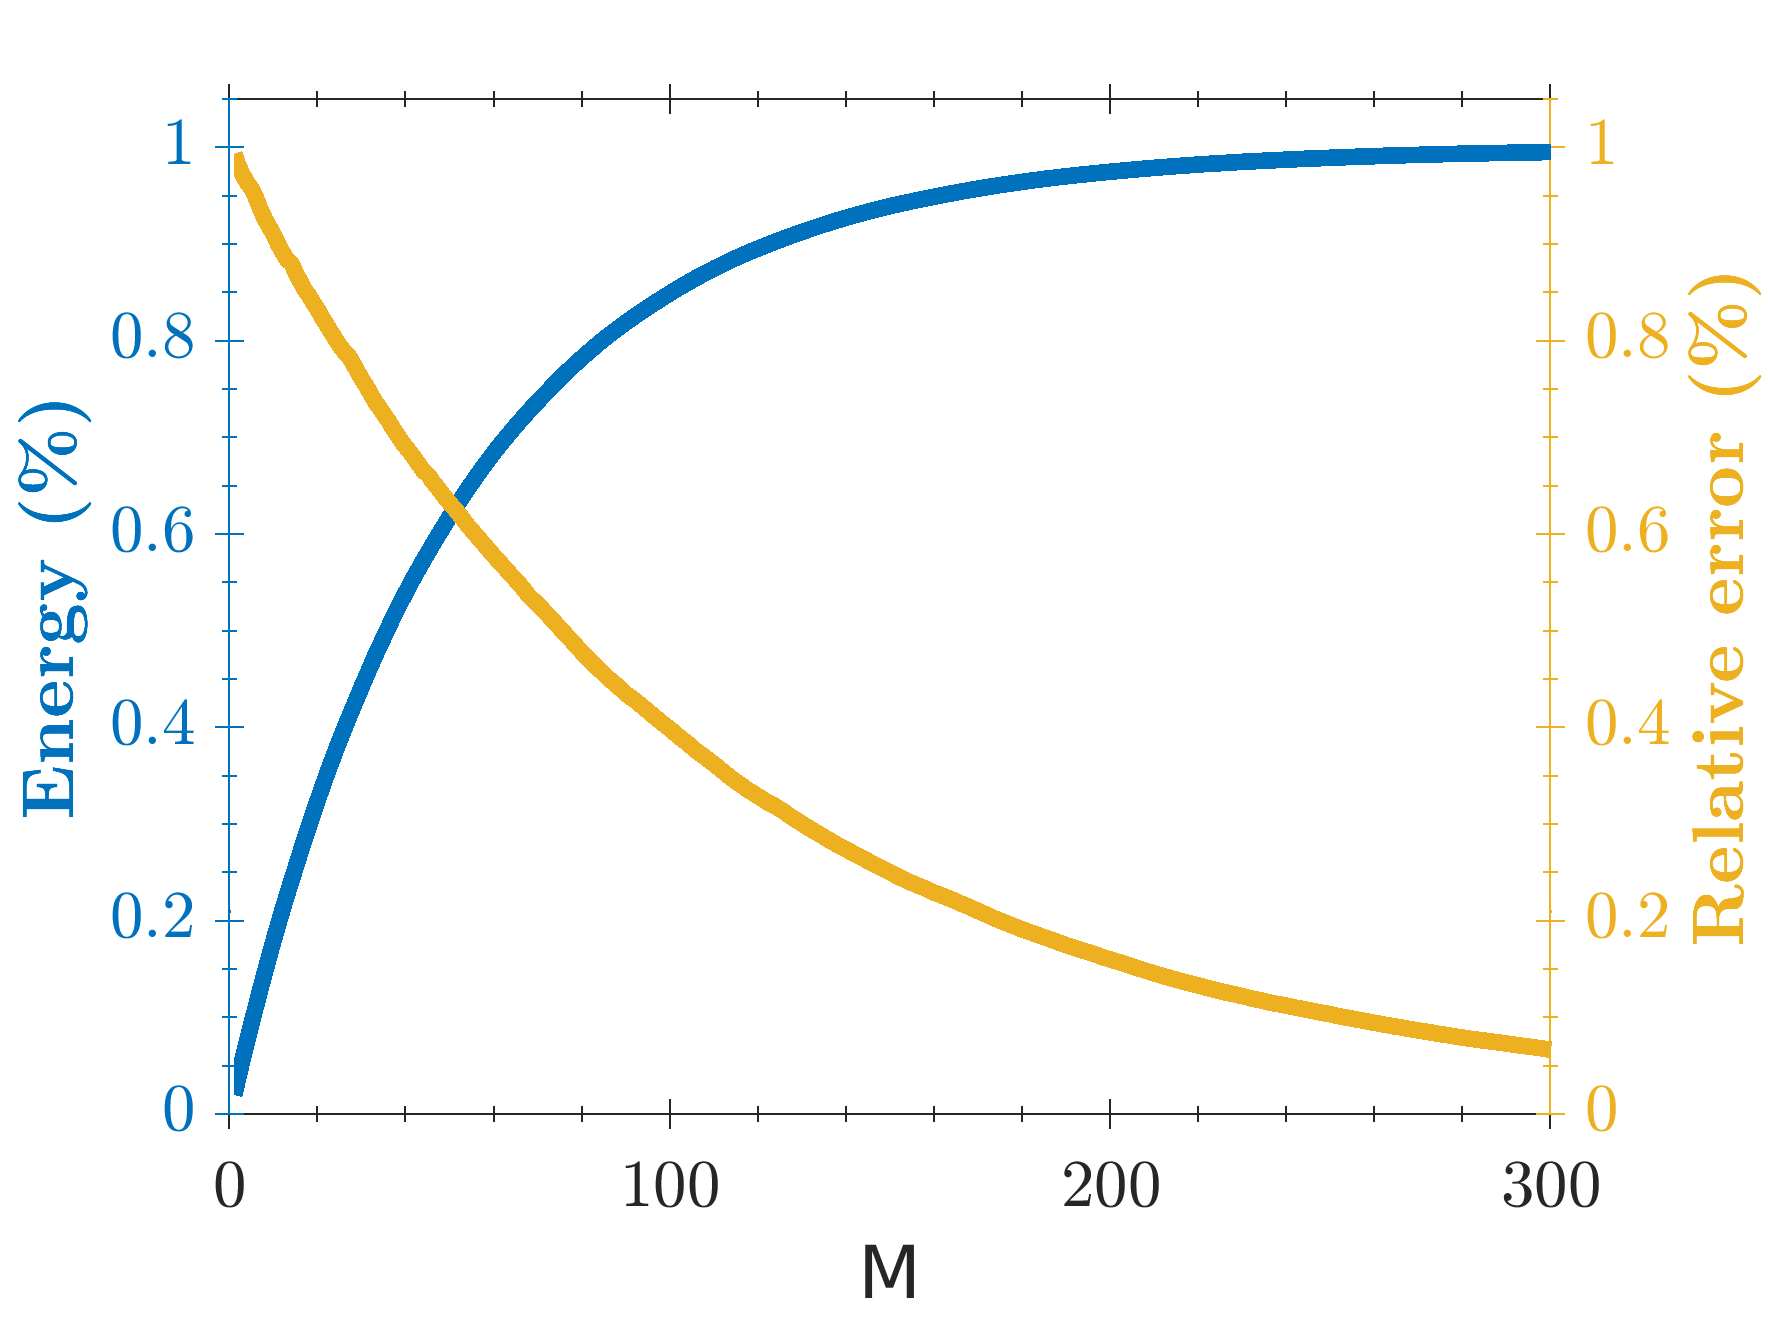
\includegraphics[scale=0.475]{./figuras/Energy_sexp_100x100x1_0-1x0-1_30000.png}
 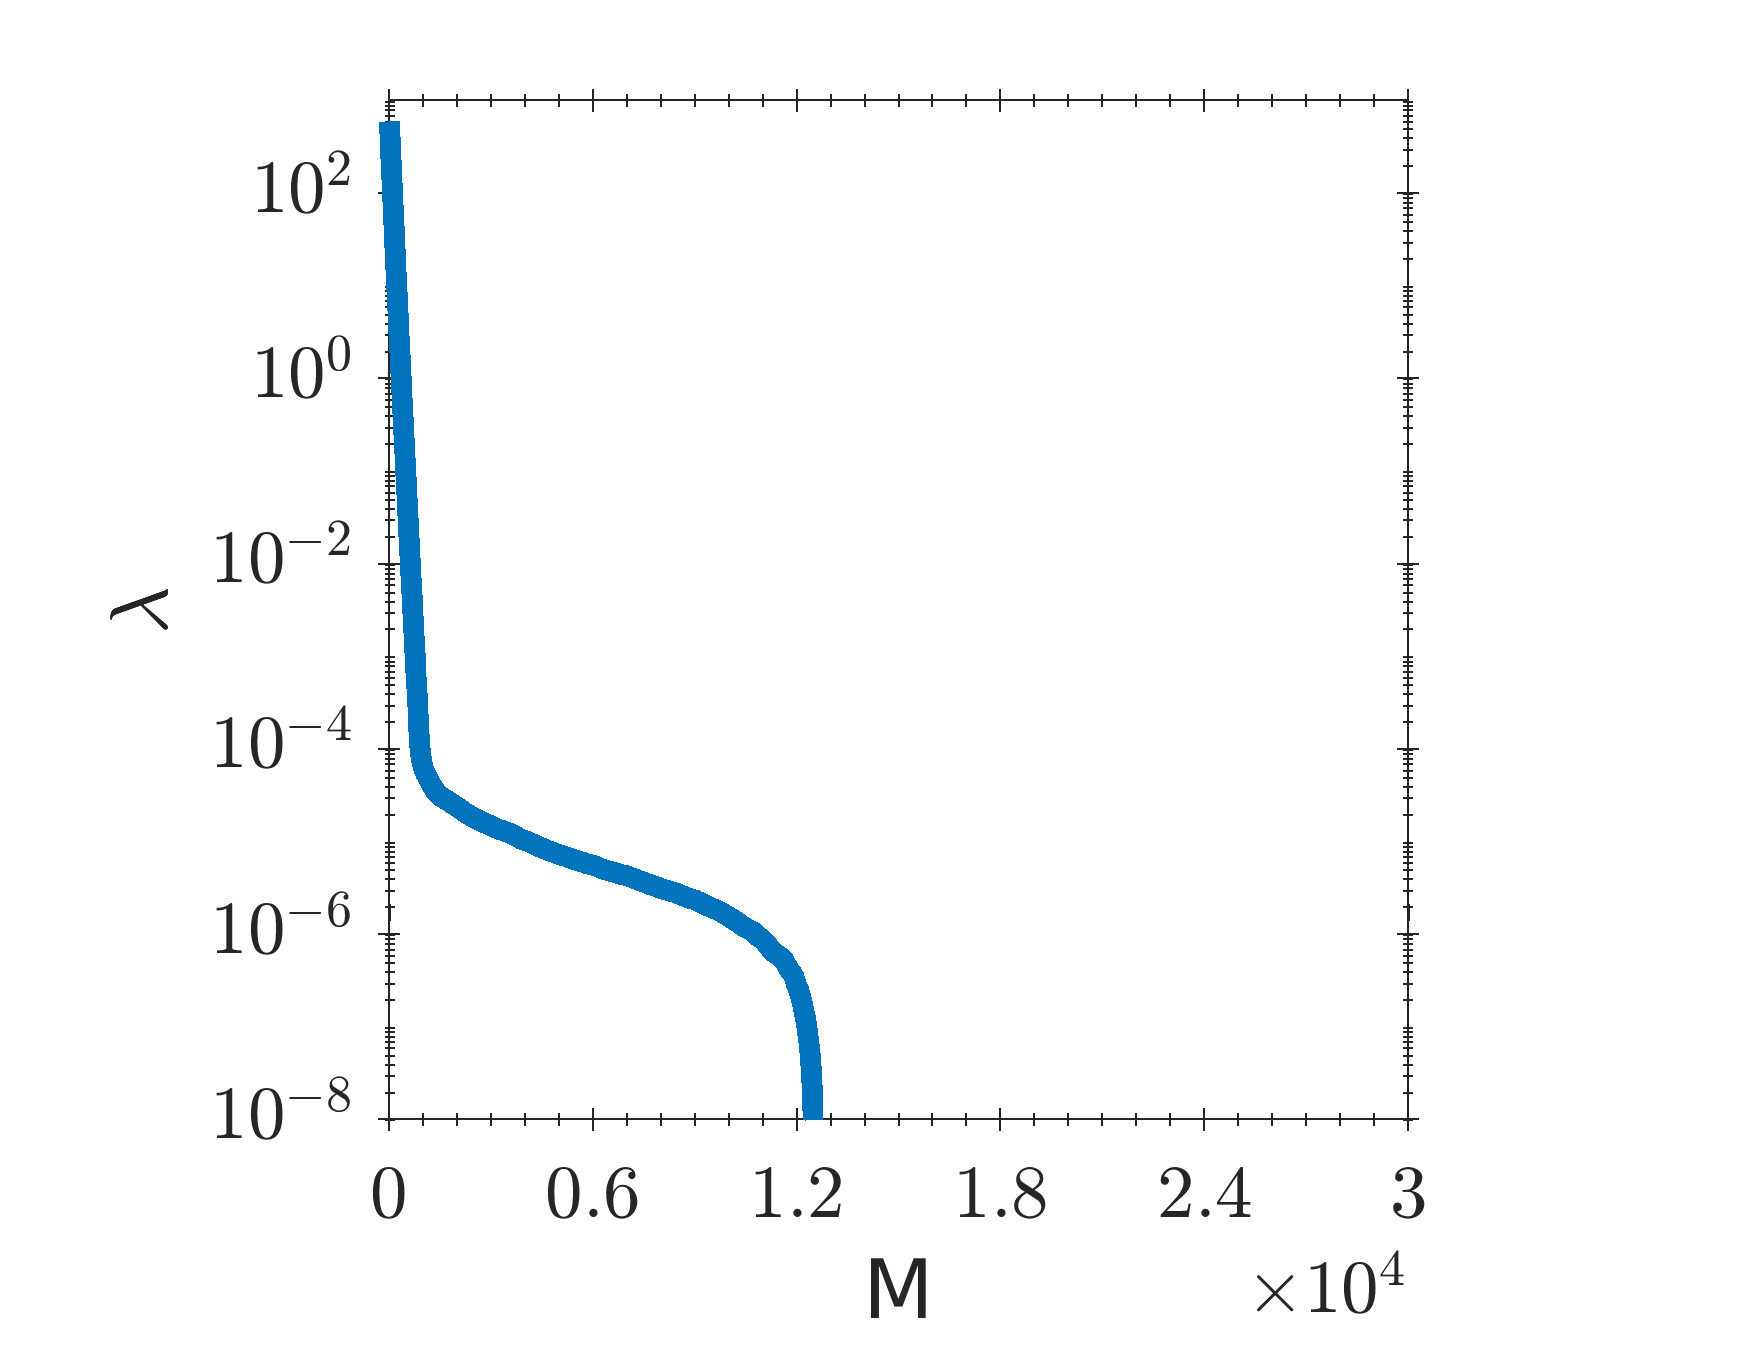
\includegraphics[scale=0.485]{./figuras/sexp_autoval_100x100x1_0-1x0-1_30000.png}}
 \subfigure[Exponential covariance ($\clen= 0.1$)]{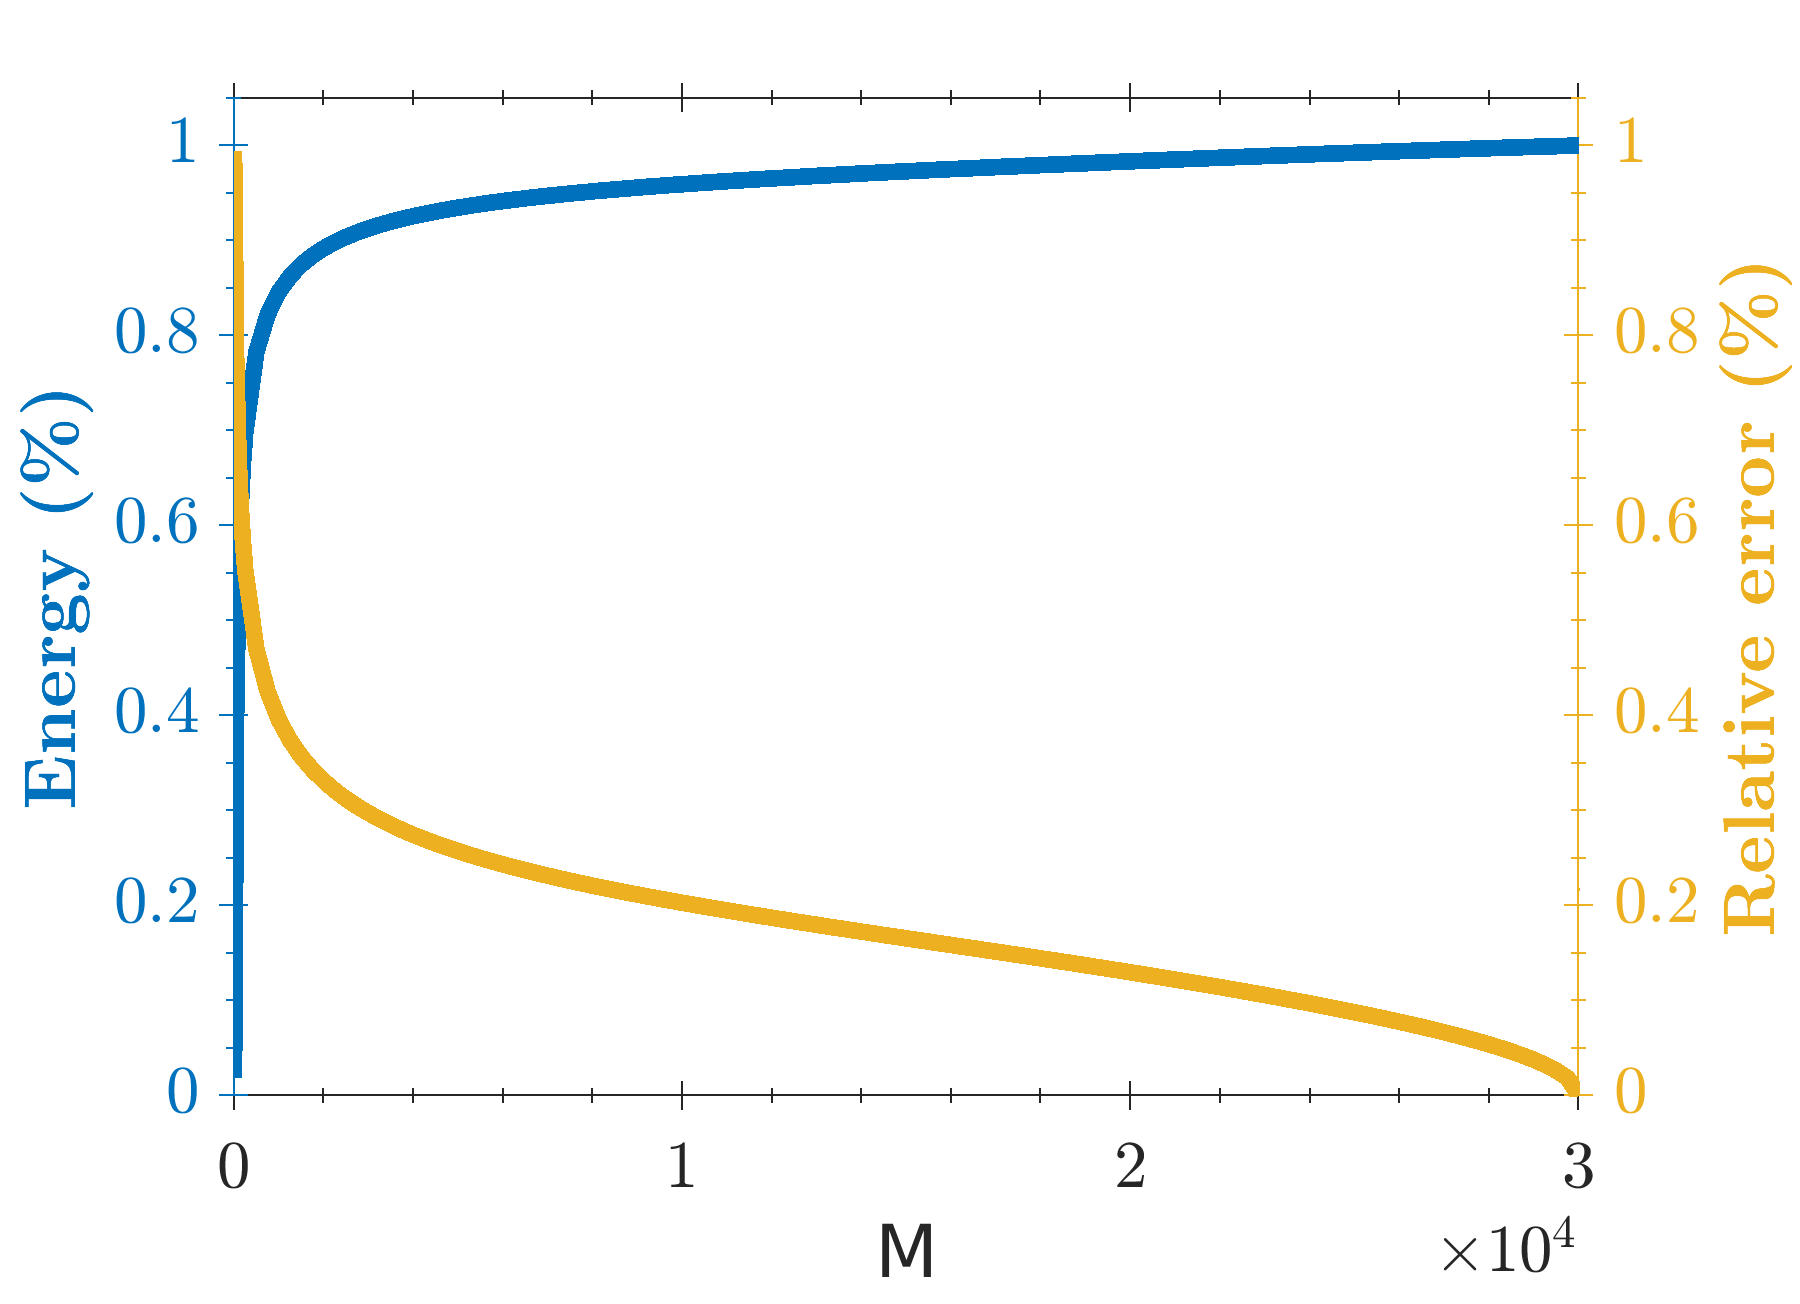
\includegraphics[scale=0.475]{./figuras/Energy_exp_100x100x1_0-1x0-1_30000.png}
 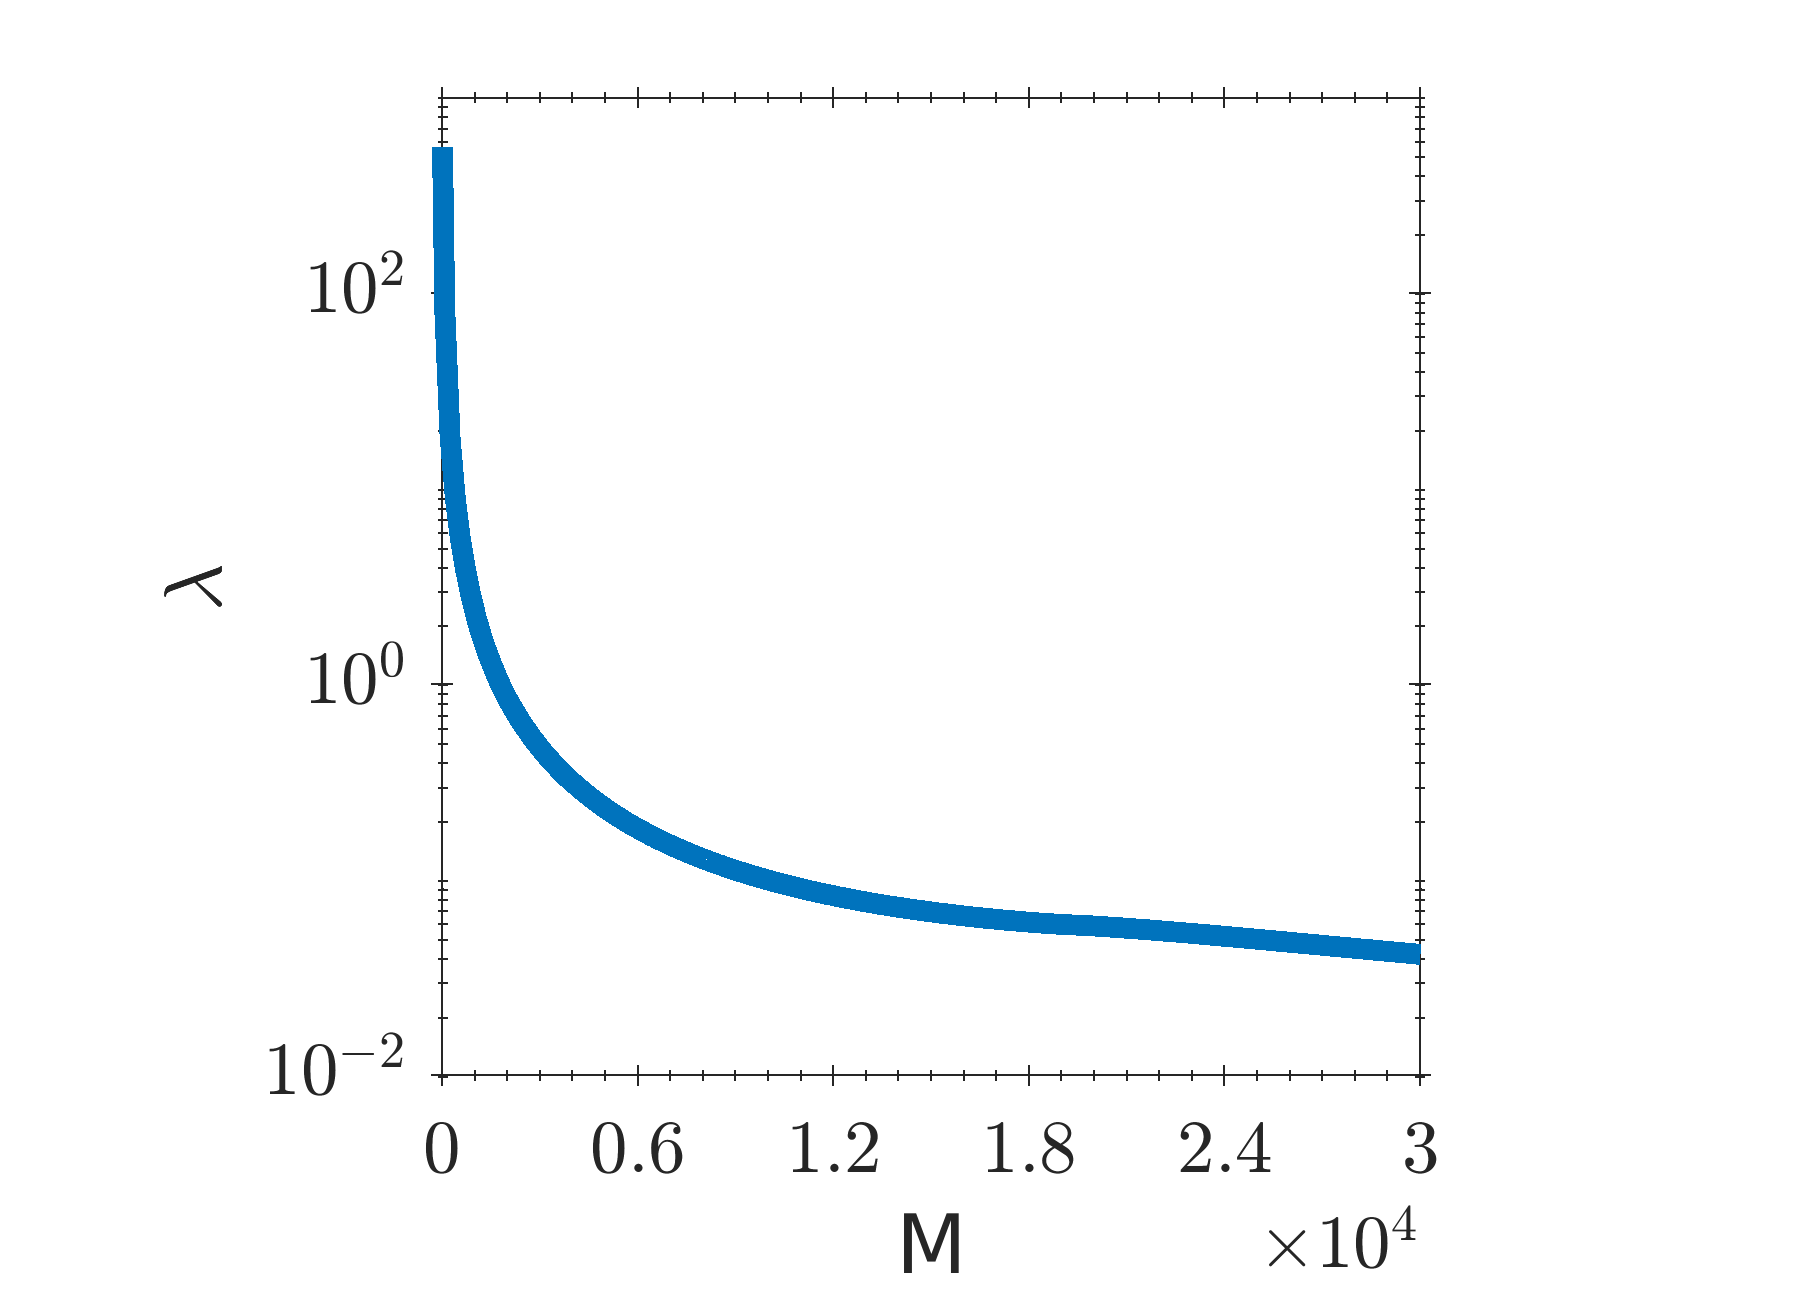
\includegraphics[scale=0.485]{./figuras/exp_autoval_100x100x1_0-1x0-1_30000.png}}\\
 \subfigure[Exponential covariance ($\clen= 0.2$)]{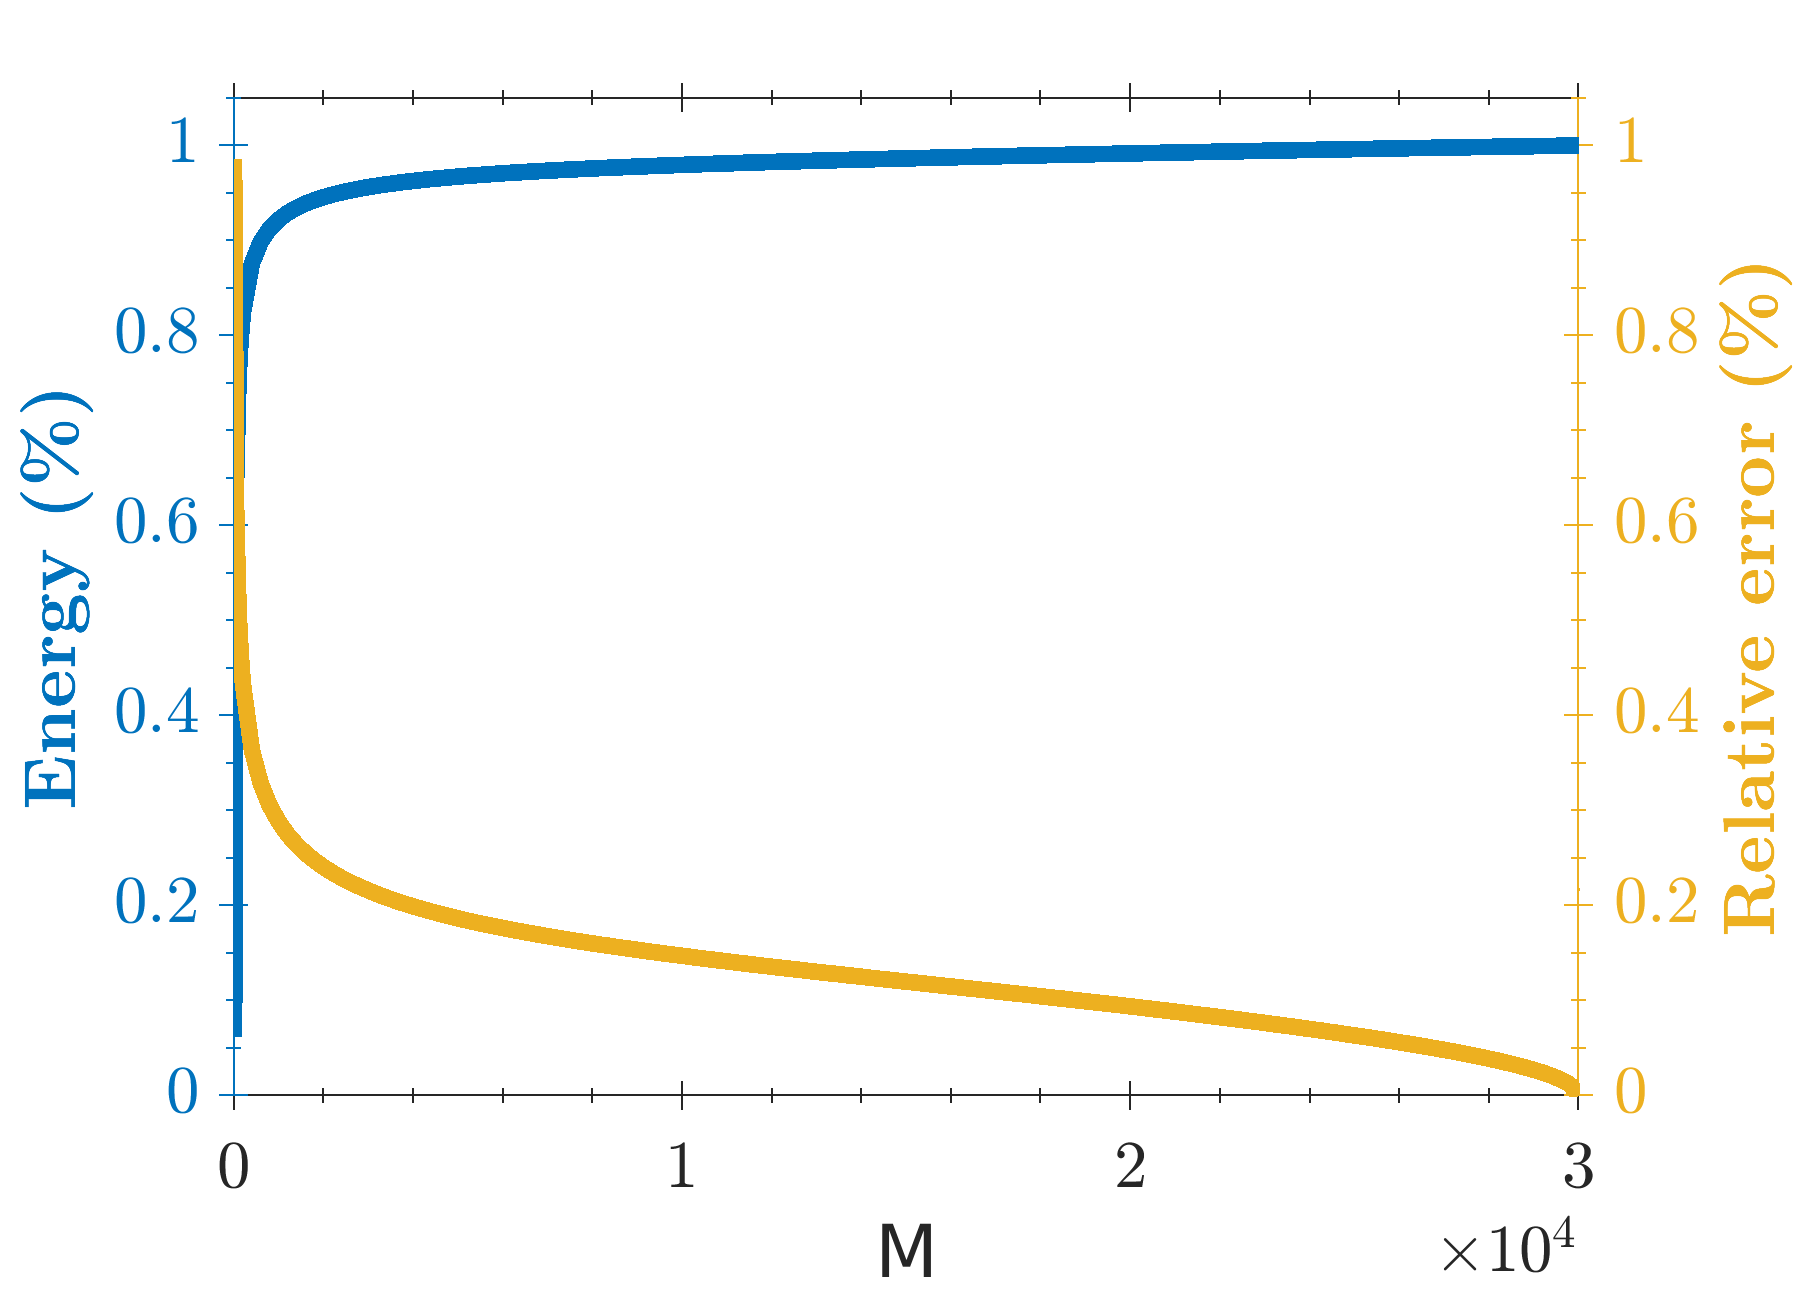
\includegraphics[scale=0.475]{./figuras/Energy_exp_100x100x1_0-2x0-2_30000.png}
 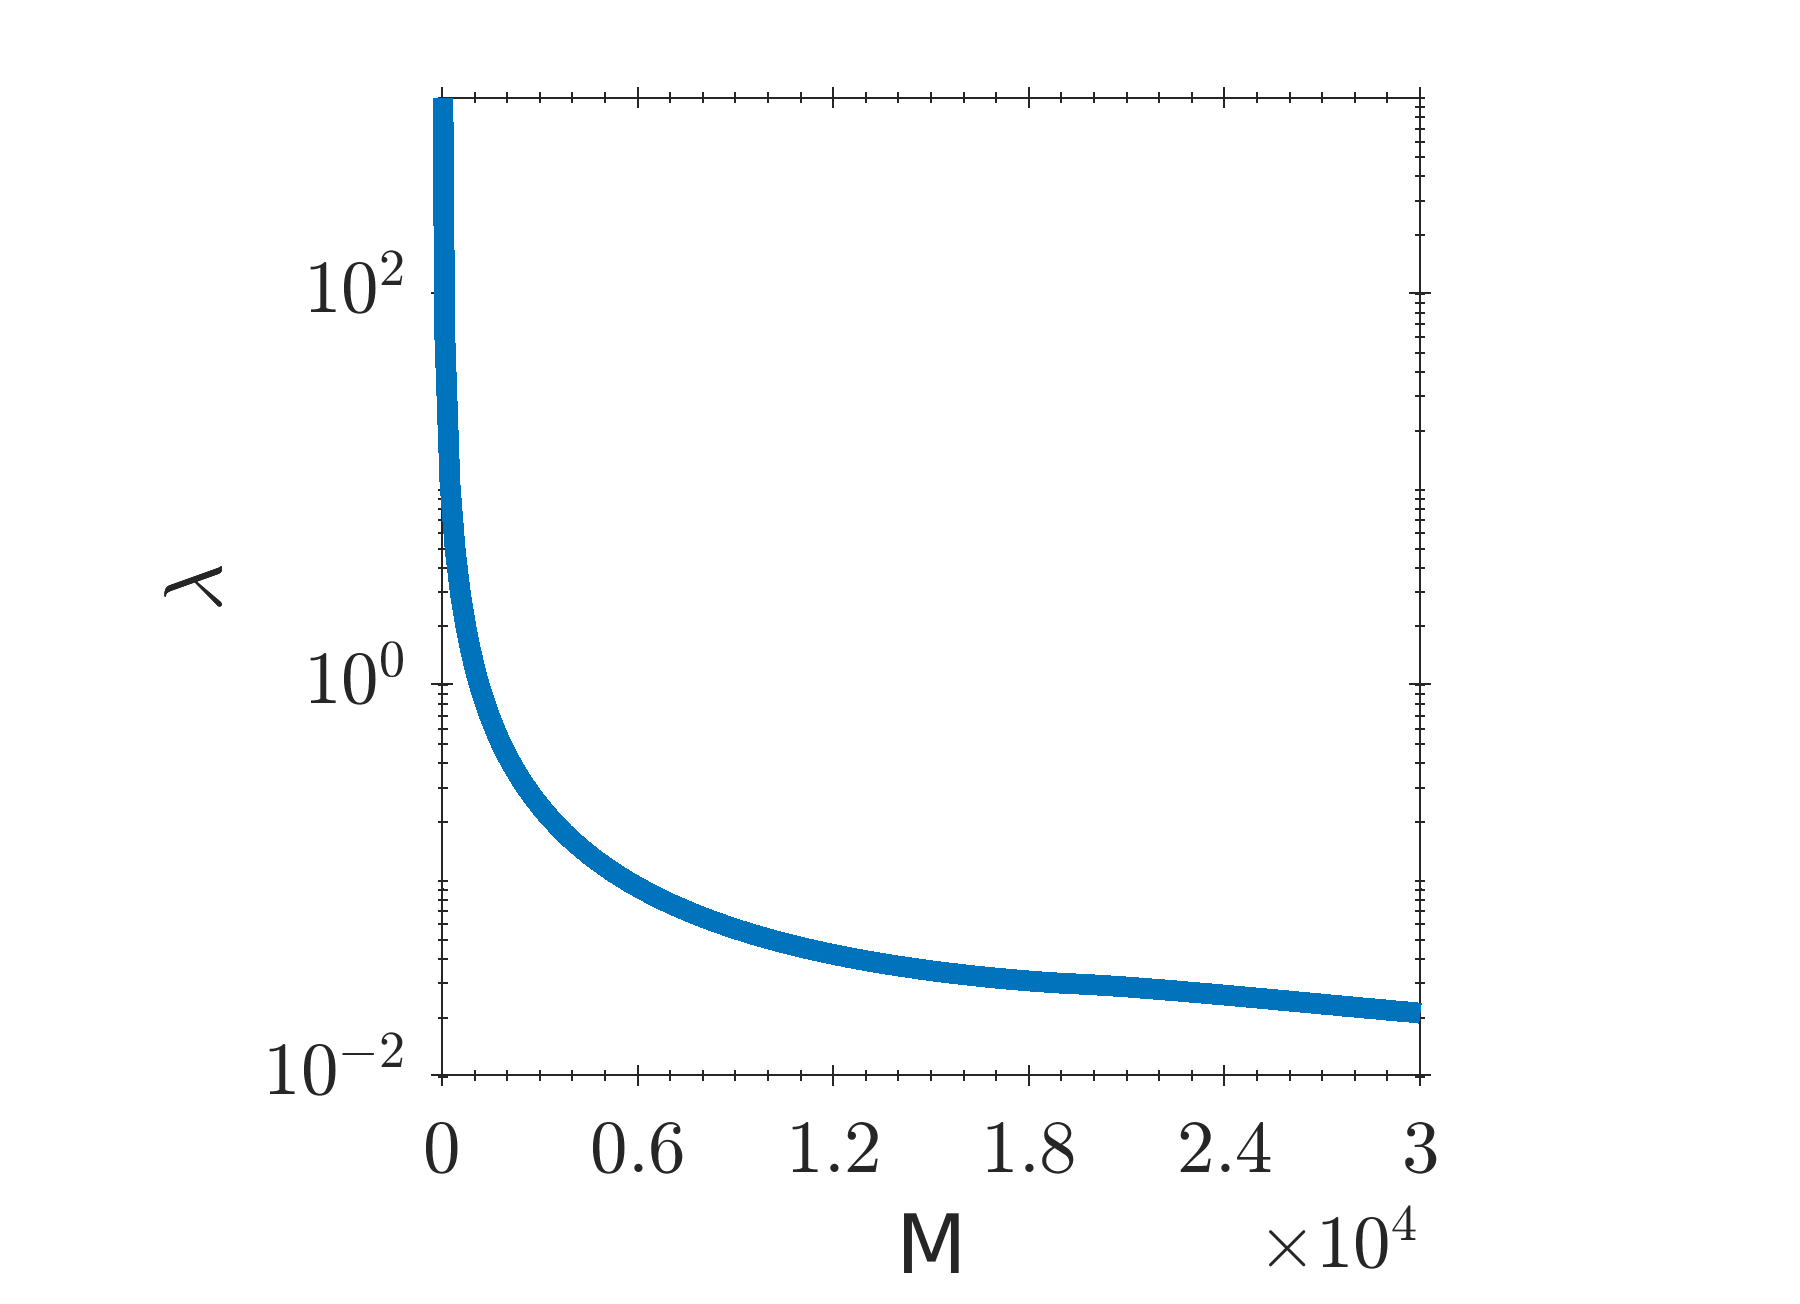
\includegraphics[scale=0.485]{./figuras/exp_autoval_100x100x1_0-2x0-2_30000.png}}
 \caption{Decay of eigenvalues and contained energy as a function of the number of terms in the expansion.}
 \label{eigenvalues}
\end{figure}


%%%%%%%%%%%%%%%%%%%%%%%%%%%%%%%%%%%%%%%%%%%%%%%%%%%%%%%%%%%%%%%%%%%%%%%%%%%%%%%%%%%%%%
\begin{figure}[H]
 \centering
 \subfigure[$\En=80\%$]{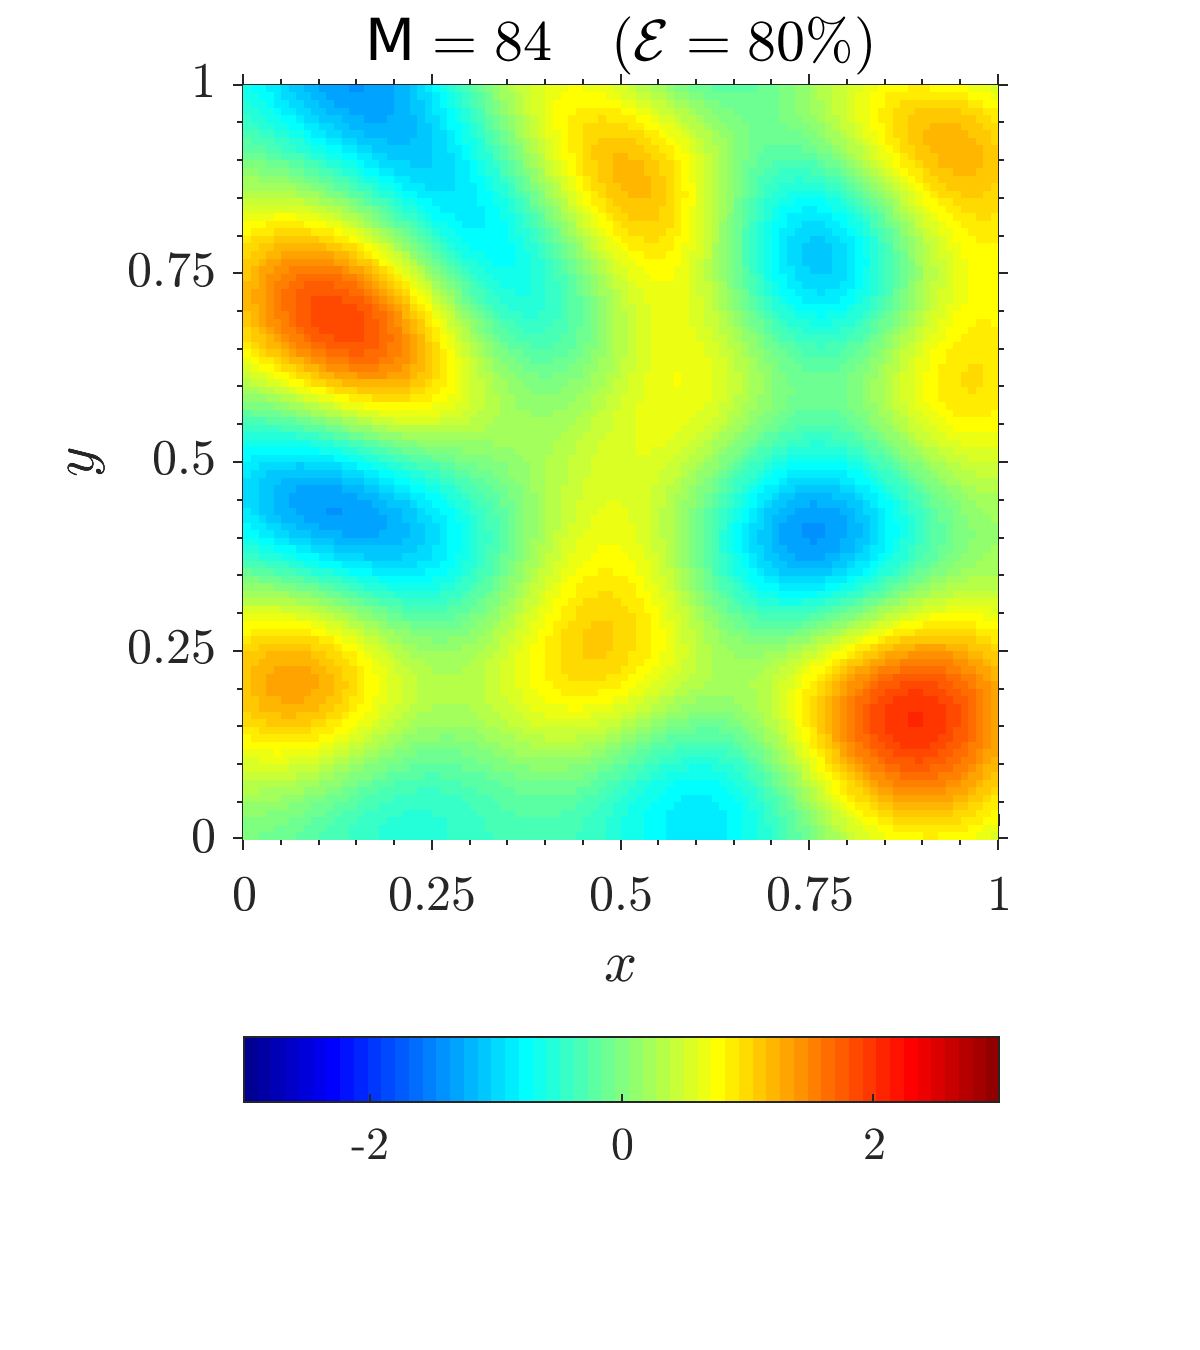
\includegraphics[scale=0.5]{figuras/Y_sexp_01_E80.png}
 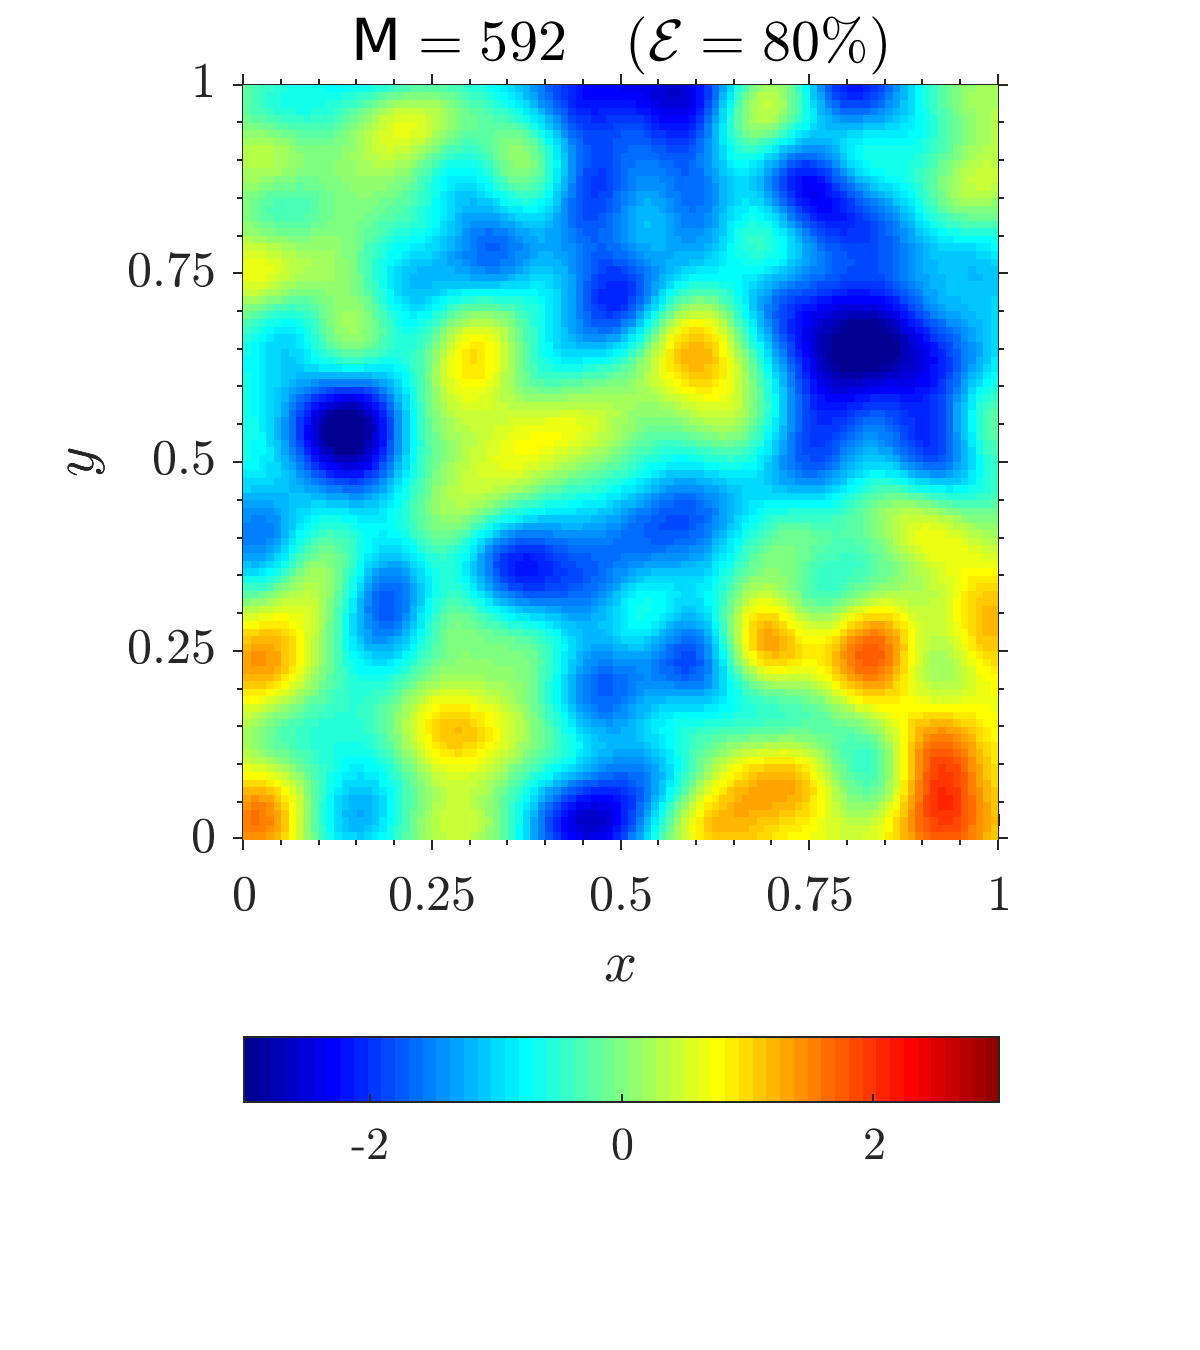
\includegraphics[scale=0.5]{figuras/Y_exp_01_E80.png}
 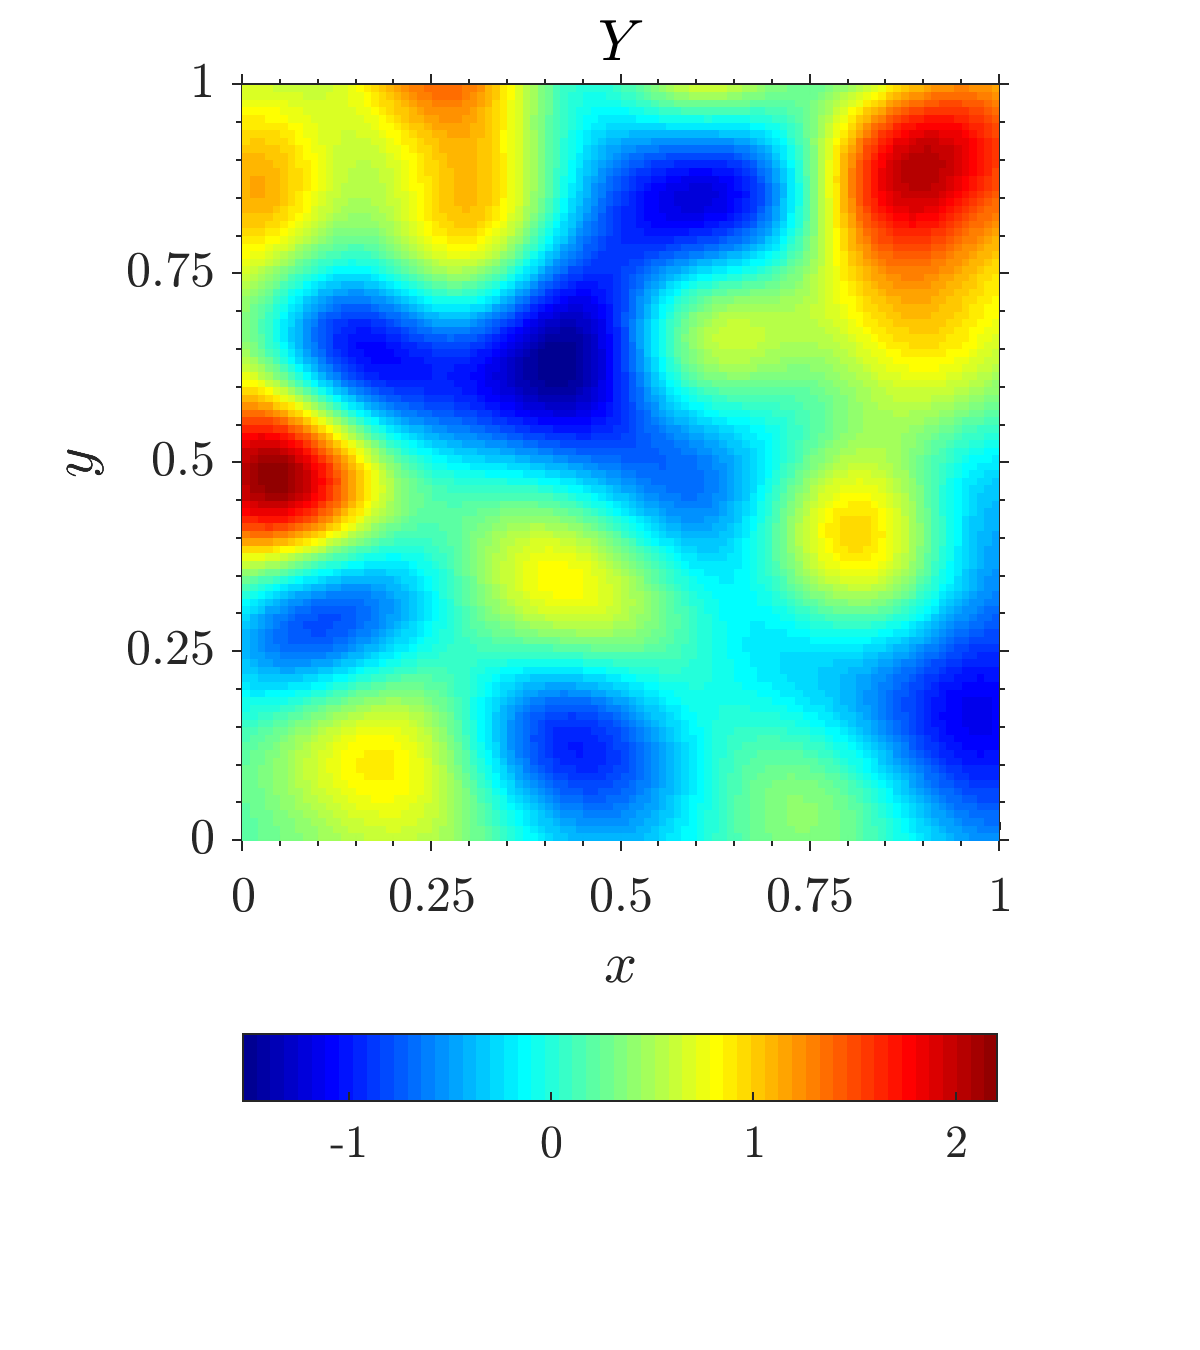
\includegraphics[scale=0.5]{figuras/Y_exp_02_E80.png}}
 \subfigure[$\En=96\%$]{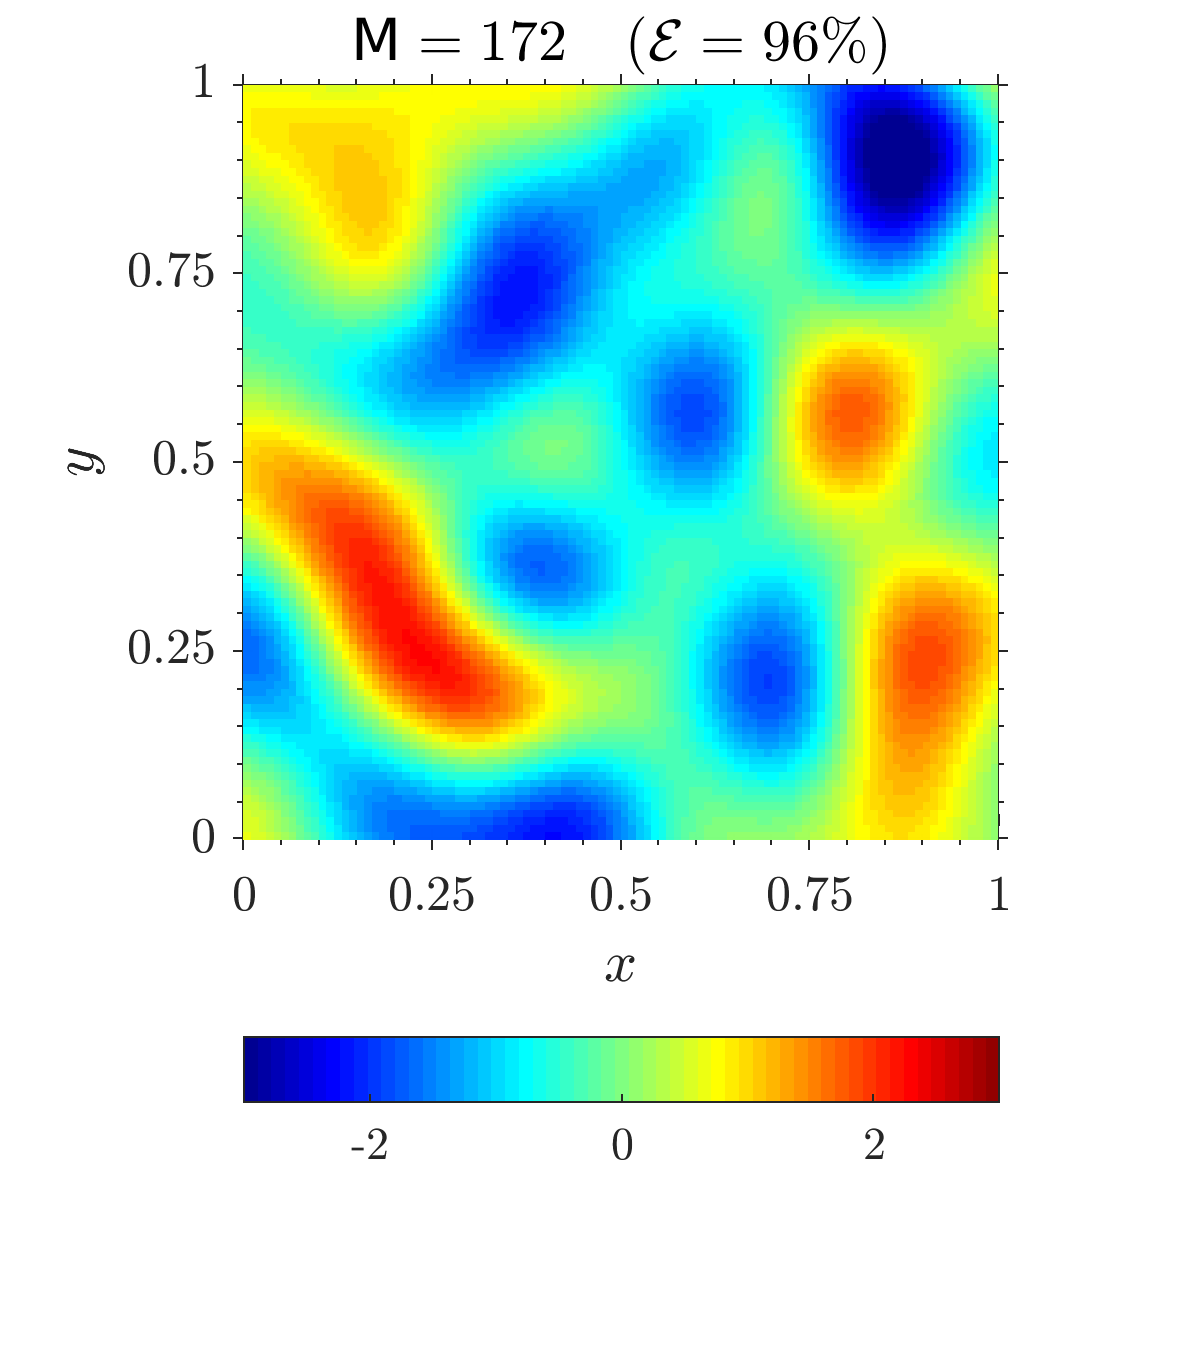
\includegraphics[scale=0.5]{figuras/Y_sexp_01_E96.png}
 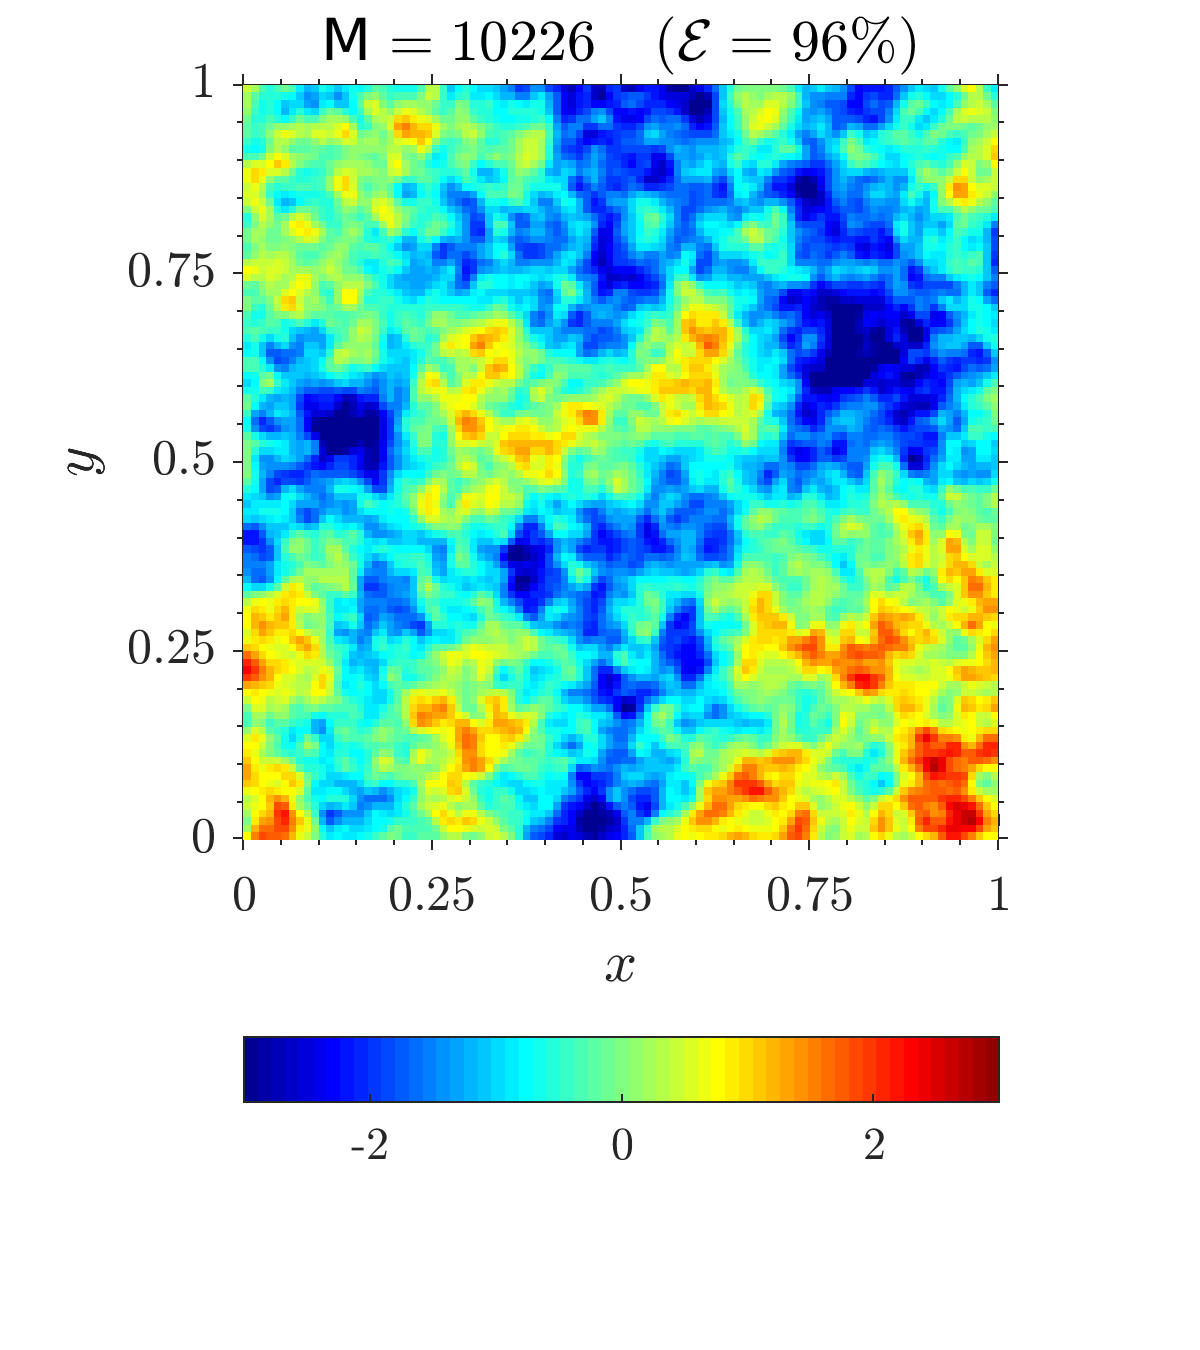
\includegraphics[scale=0.5]{figuras/Y_exp_01_E96.png}
 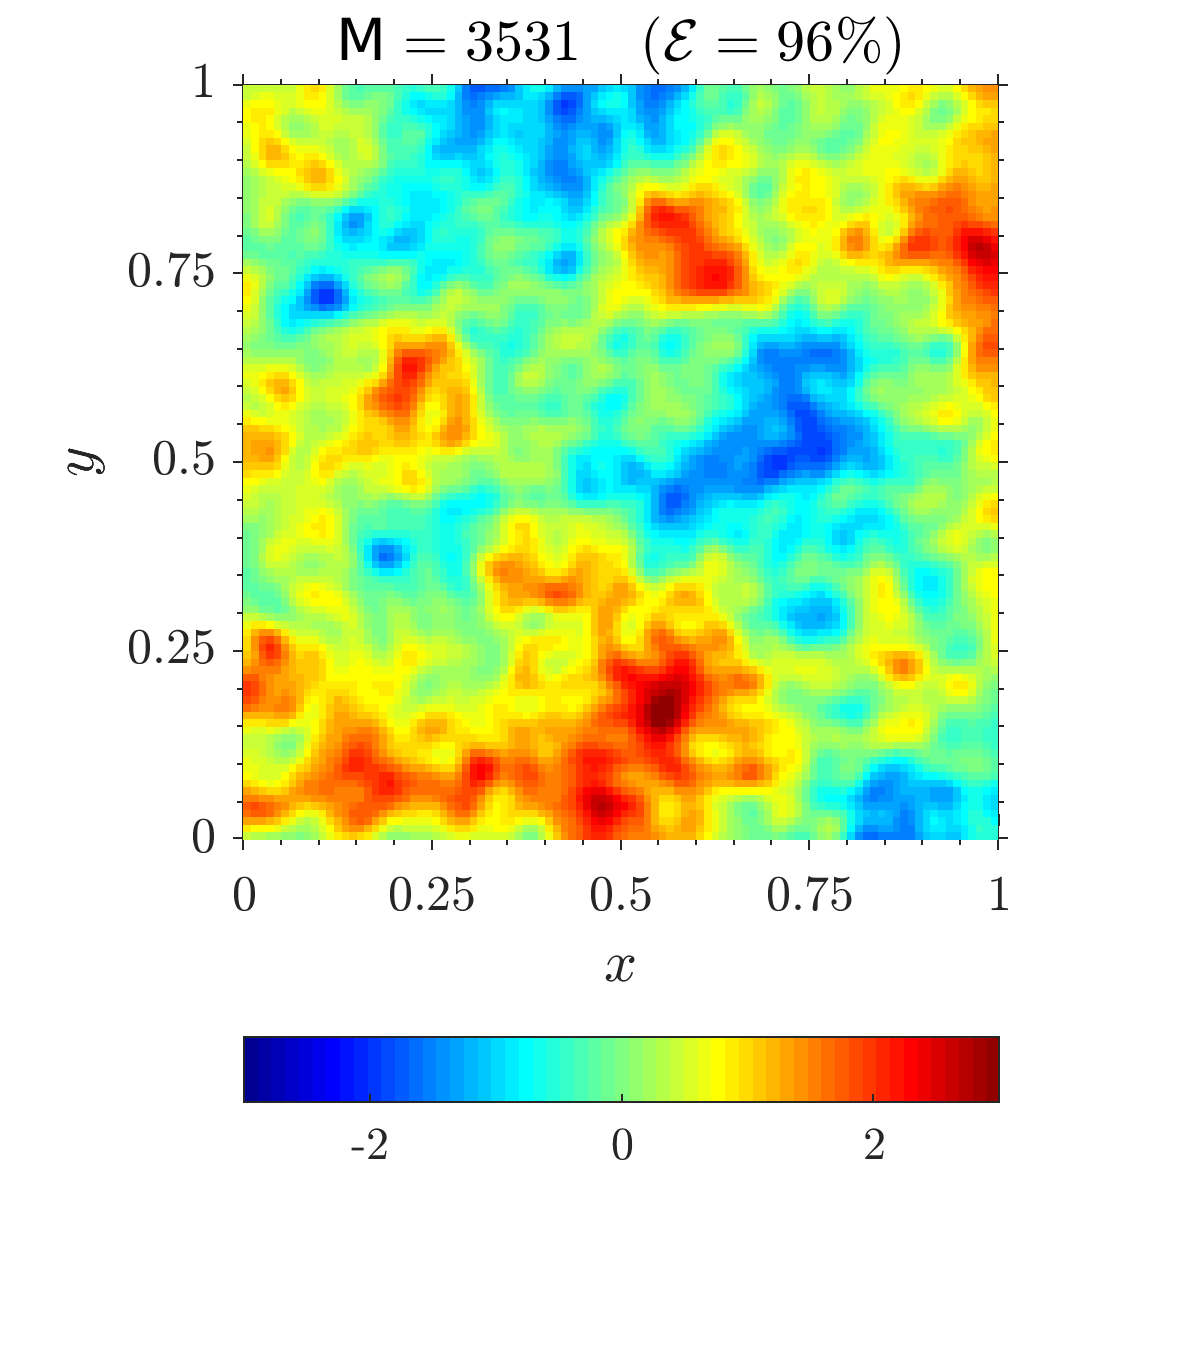
\includegraphics[scale=0.5]{figuras/Y_exp_02_E96.png}}
 \subfigure[$\En\sim 100\%$]{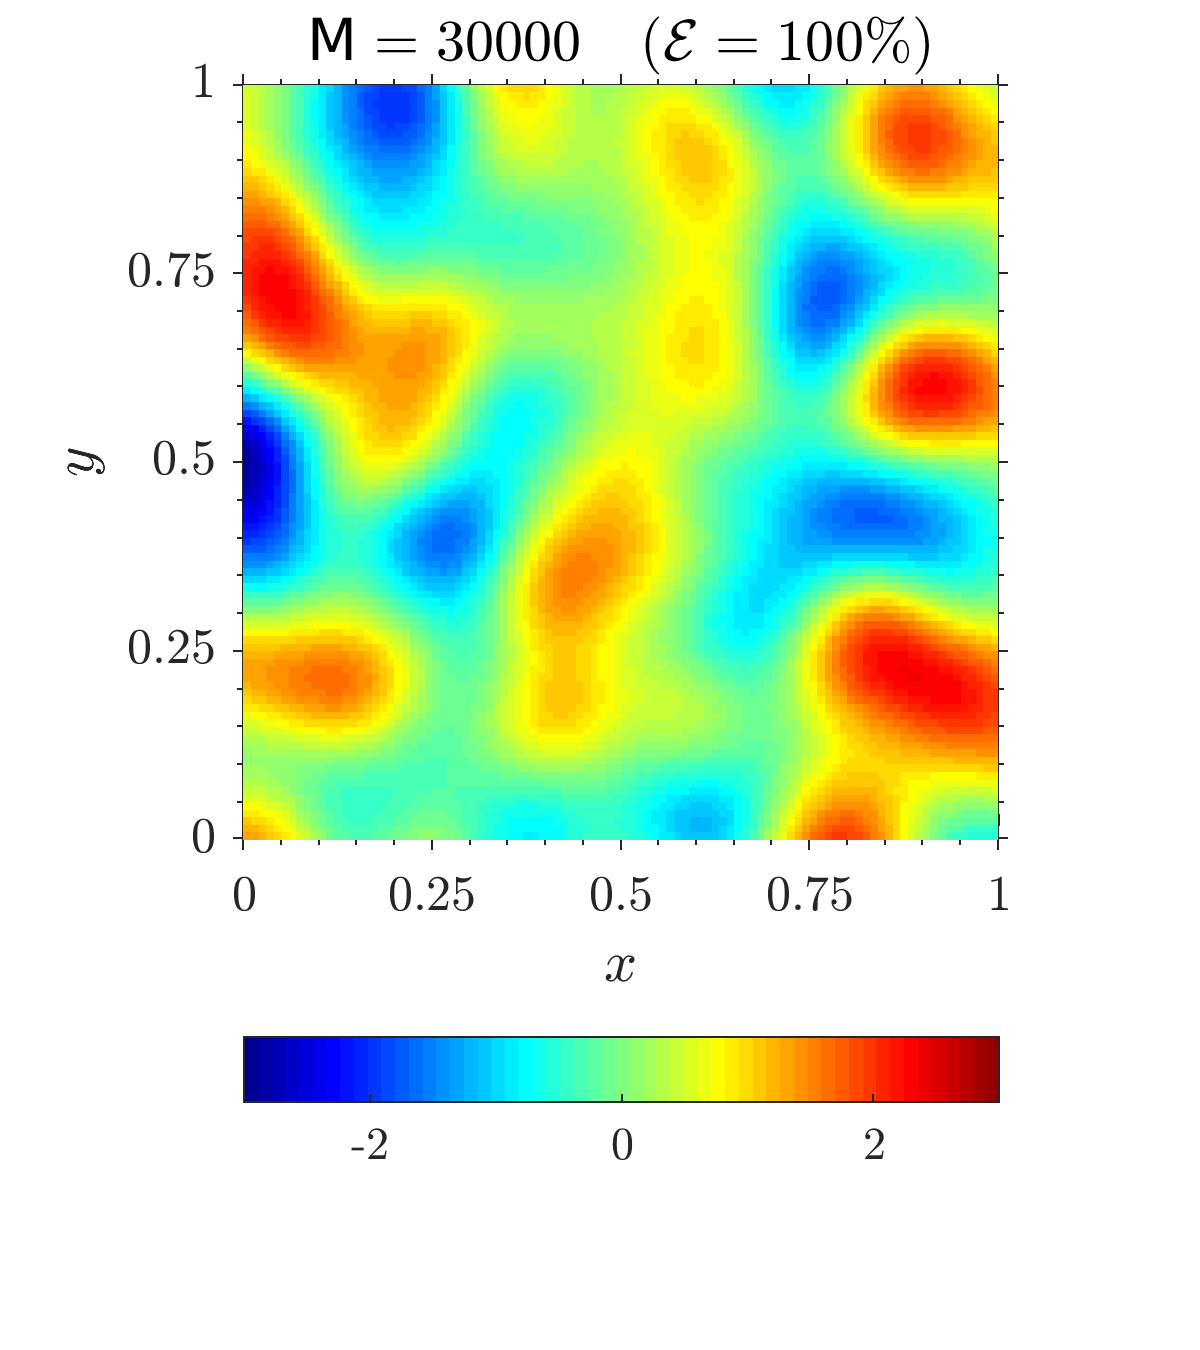
\includegraphics[scale=0.5]{figuras/Y_sexp_01_E100.png}
 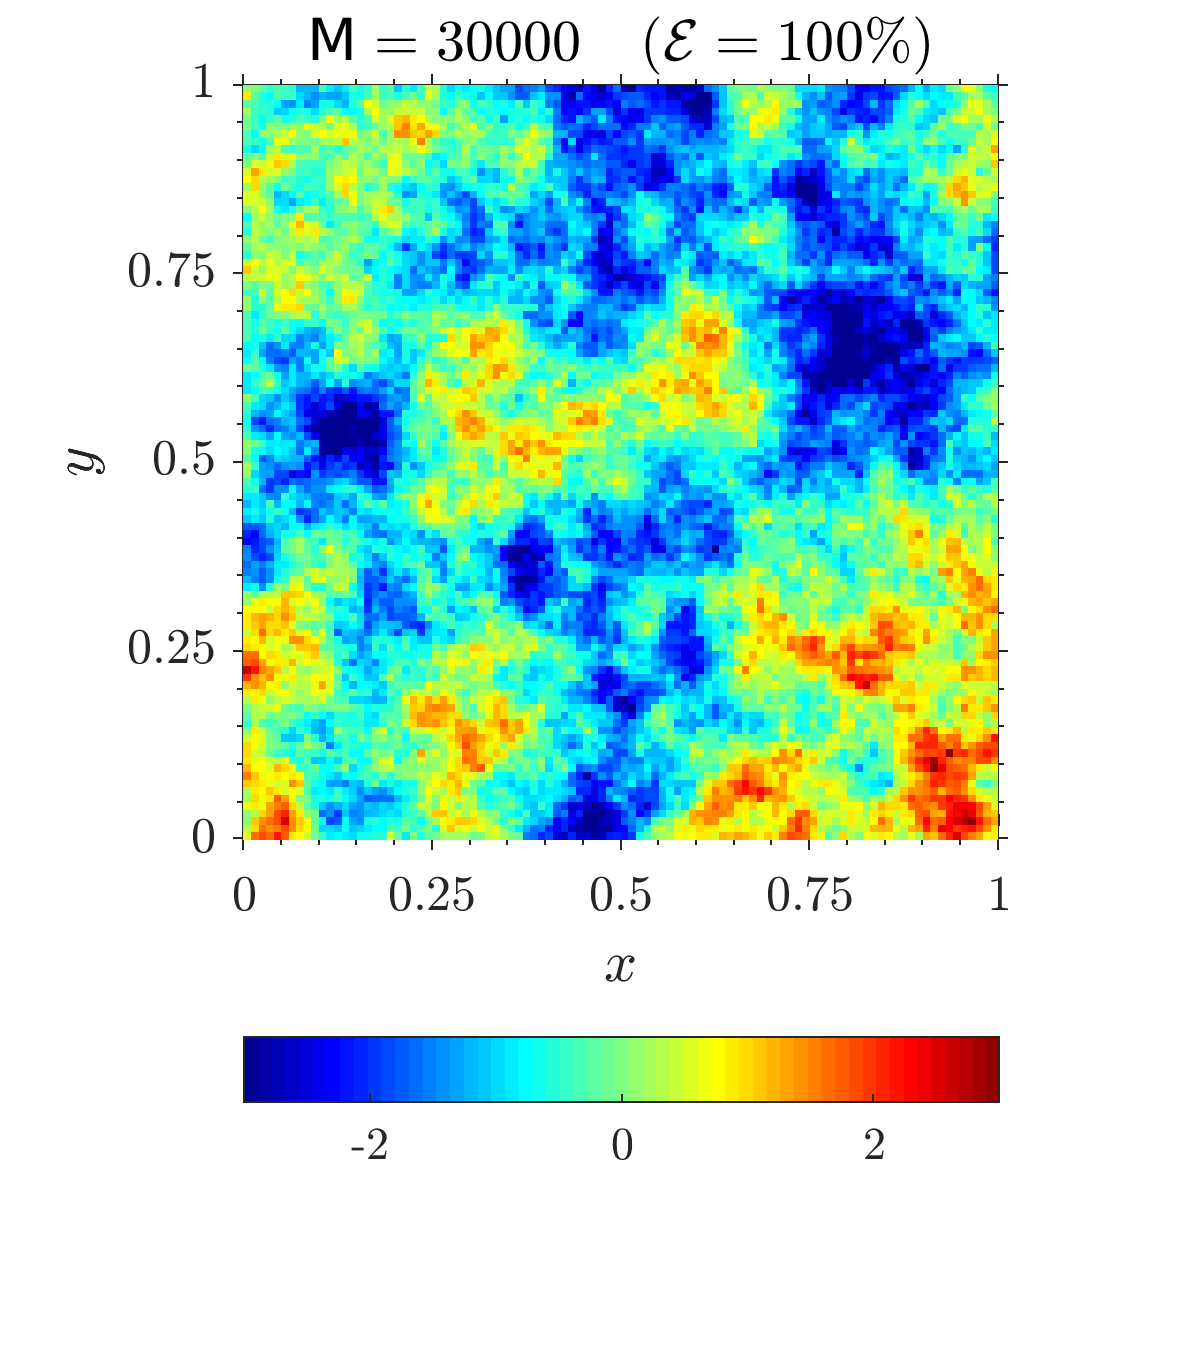
\includegraphics[scale=0.5]{figuras/Y_exp_01_E100.png}
 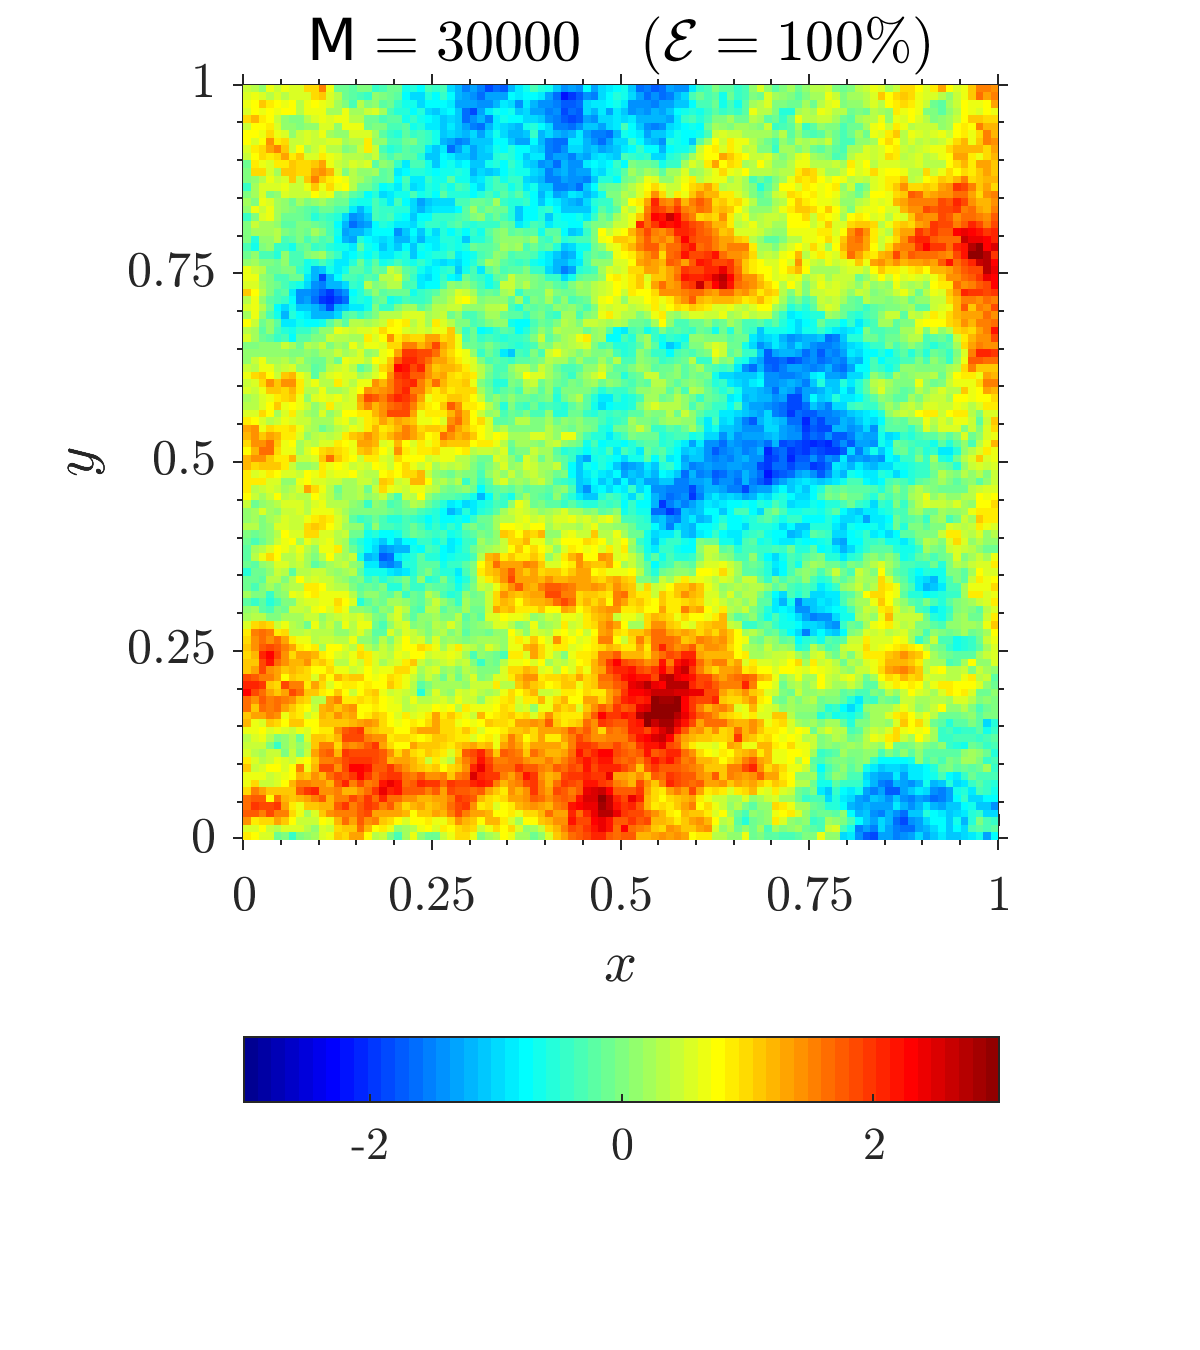
\includegraphics[scale=0.5]{figuras/Y_exp_02_E100.png}}
\end{figure}

%%%%%%%%%%%%%%%%%%%%%%%%%%%%%%%%%%%%%%%%%%%%%%%%%%%%%%%%%%%%%%%%%%%%%%%%%%%%%%%%%%%%%%

\begin{table}[H]
\caption{Number of \kl\ expansion terms needed to obtain an given energy level}
\label{tab:KLE}
{
\newcommand{\mc}[3]{\multicolumn{#1}{#2}{#3}}
\begin{center}
\begin{tabular}{lccc|ccc}\hline\hline
\cline{1-7}
\mc{1}{l|}{\textbf{Energy}} & \mc{3}{c|}{$\m$} & \mc{3}{c}{\textbf{Mean relative error}}\\\cline{2-7}
\mc{1}{l|}{\textbf{}} & Squared Exp. & Exponential & Exponential & Squared Exp. & Exponential & Exponential \\
\mc{1}{l|}{\textbf{($\%$)}} & ($\clen=0.1$) & ($\clen=0.1$) & ($\clen=0.2$) & ($\clen=0.1$) & ($\clen=0.1$) & ($\clen=0.2$)\\\hline
\mc{1}{l|}{\textbf{80}} & 84  & 592   & 154 & 0.46 & 0.45 & 0.47\\
\mc{1}{l|}{\textbf{90}} & 122 & 2,323  & 612 & 0.32 & 0.32 & 0.33\\
\mc{1}{l|}{\textbf{94}} & 150 & 5,760  & 1,655 & 0.25 & 0.25 & 0.25\\
\mc{1}{l|}{\textbf{96}} & 172 & 10,226 & 3,531 & 0.21 & 0.20 & 0.21\\
\mc{1}{l|}{\textbf{98}} & 211 & 18,327 & 10,239 & 0.14 & 0.14 & 0.15\\
\mc{1}{l|}{\textbf{100}}& $\sim$30,000 & $\sim$30,000 & $\sim$30,000 & 0.00 & 0.00 & 0.00\\\hline\hline
 \end{tabular}
 \end{center}
}
\end{table}

%%%%%%%%%%%%%%%%%%%%%%%%%%%%%%%%%%%%%%%%%%%%%%%%%%%%%%%%%%%%%%%%%%%%%%%%%%%%%%%%%%%%%%
\begin{figure}[H]
 \centering
 \subfigure[$x$ direction]{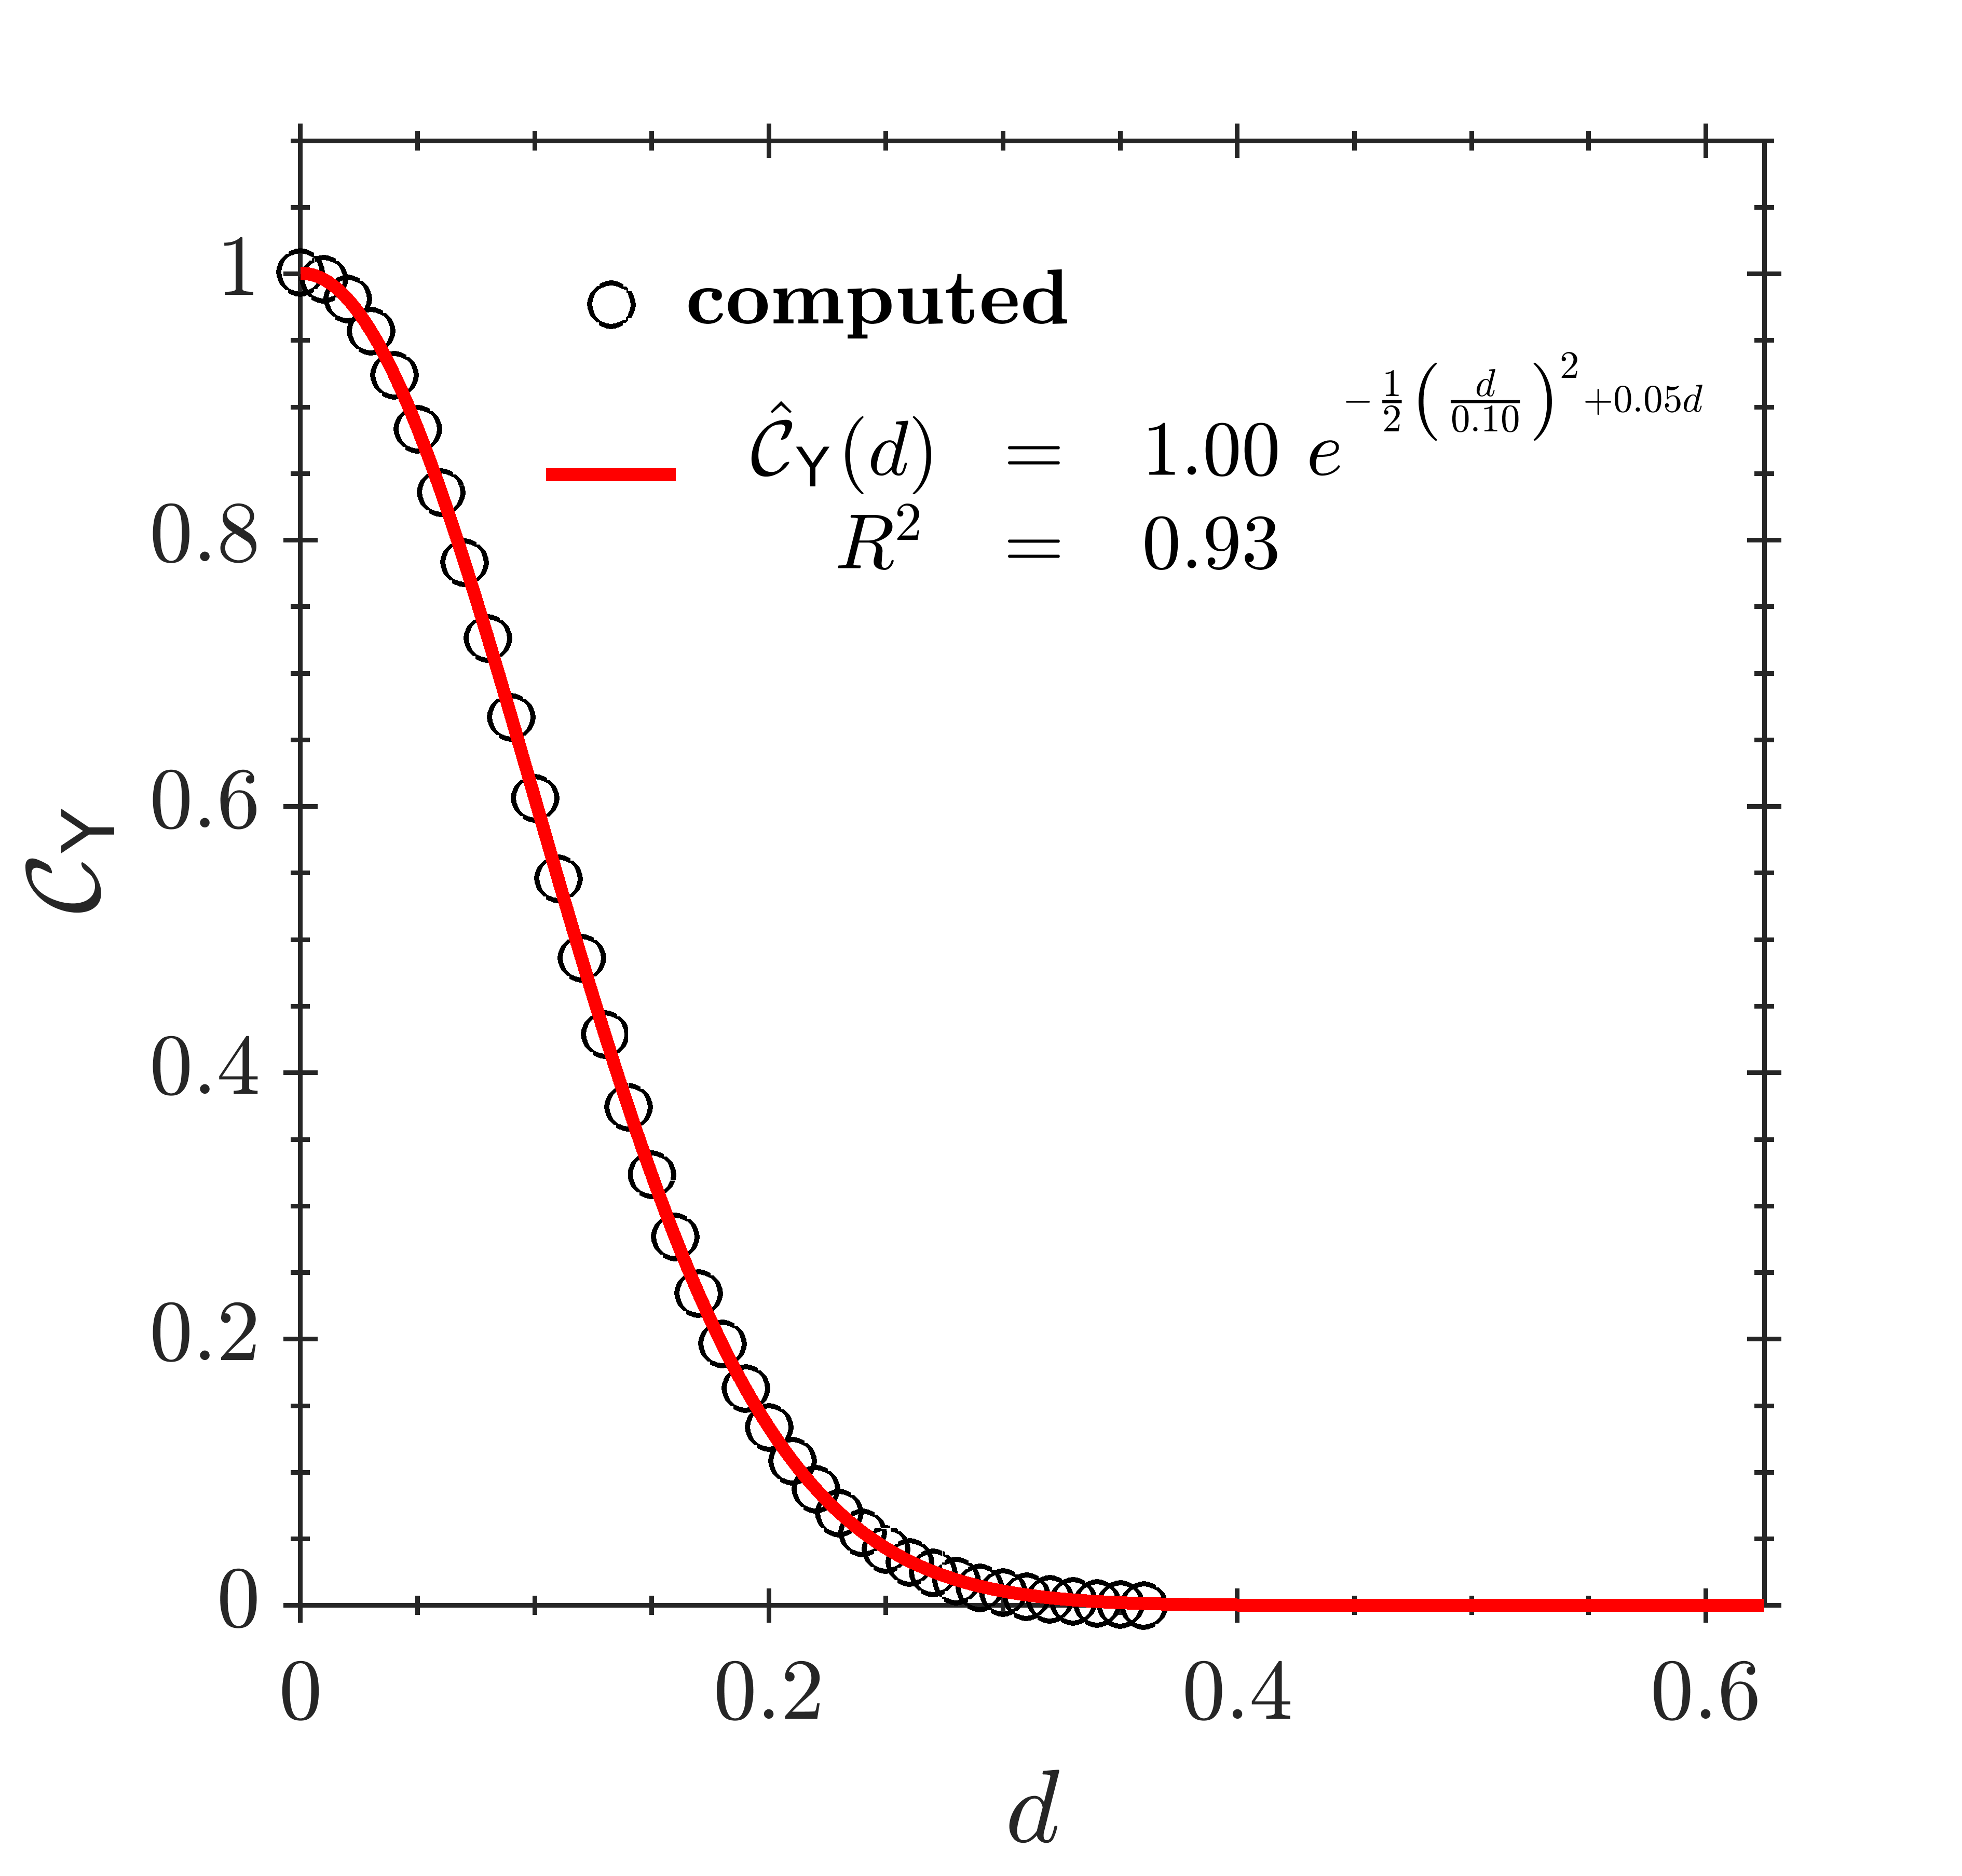
\includegraphics[scale=0.45]{./figuras/e_gssexp_1x1_100x100_0-1x0-1_5000_Yx.png}}
 \subfigure[$y$ direction]{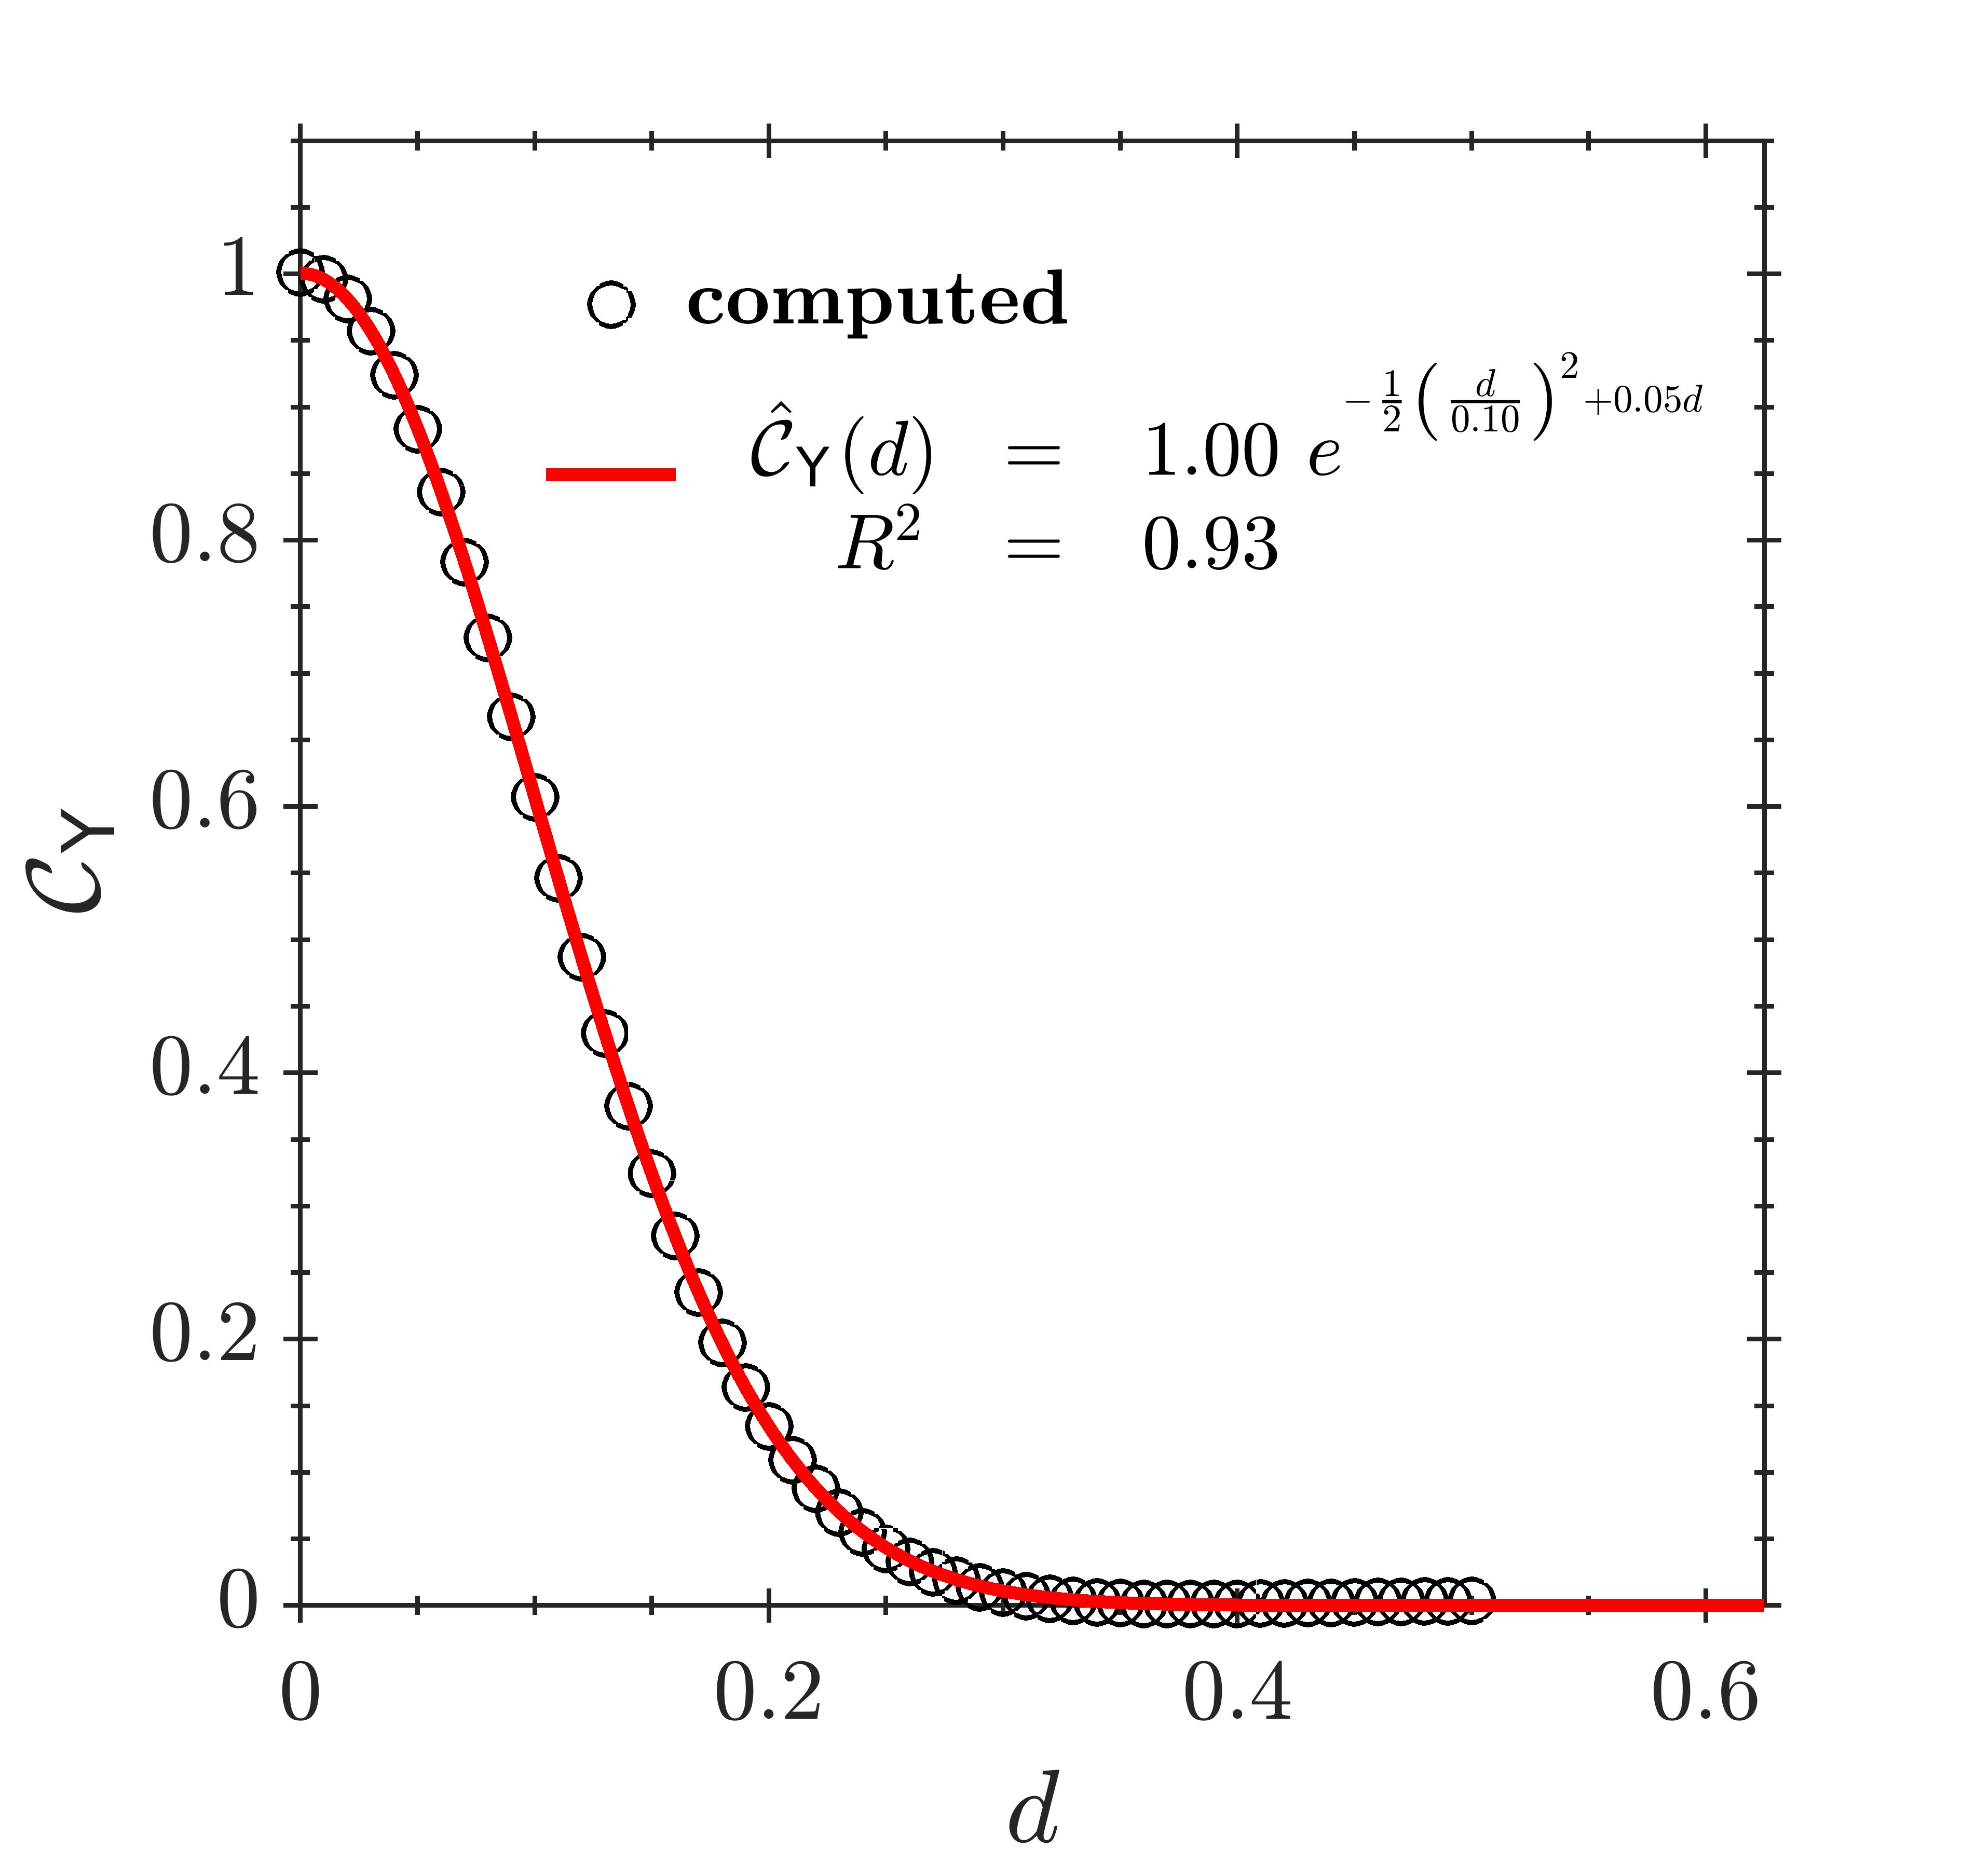
\includegraphics[scale=0.45]{./figuras/e_gssexp_1x1_100x100_0-1x0-1_5000_Yy.png}}
 \caption{Estimated covariance in a sample of $5,000$ fields generate by \kle\ with $30,000$ terms. Squared exponential case with $\clen = 0.1$.}
 \label{covar_sexpKL}
\end{figure}
%%%%%%%%%%%%%%%%%%%%%%%%%%%%%%%%%%%%%%%%%%%%%%%%%%%%%%%%%%%%%%%%%%%%%%%%%%%%%%%%%%%%%%
\begin{figure}[H]
 \centering
 \subfigure[$x$ direction]{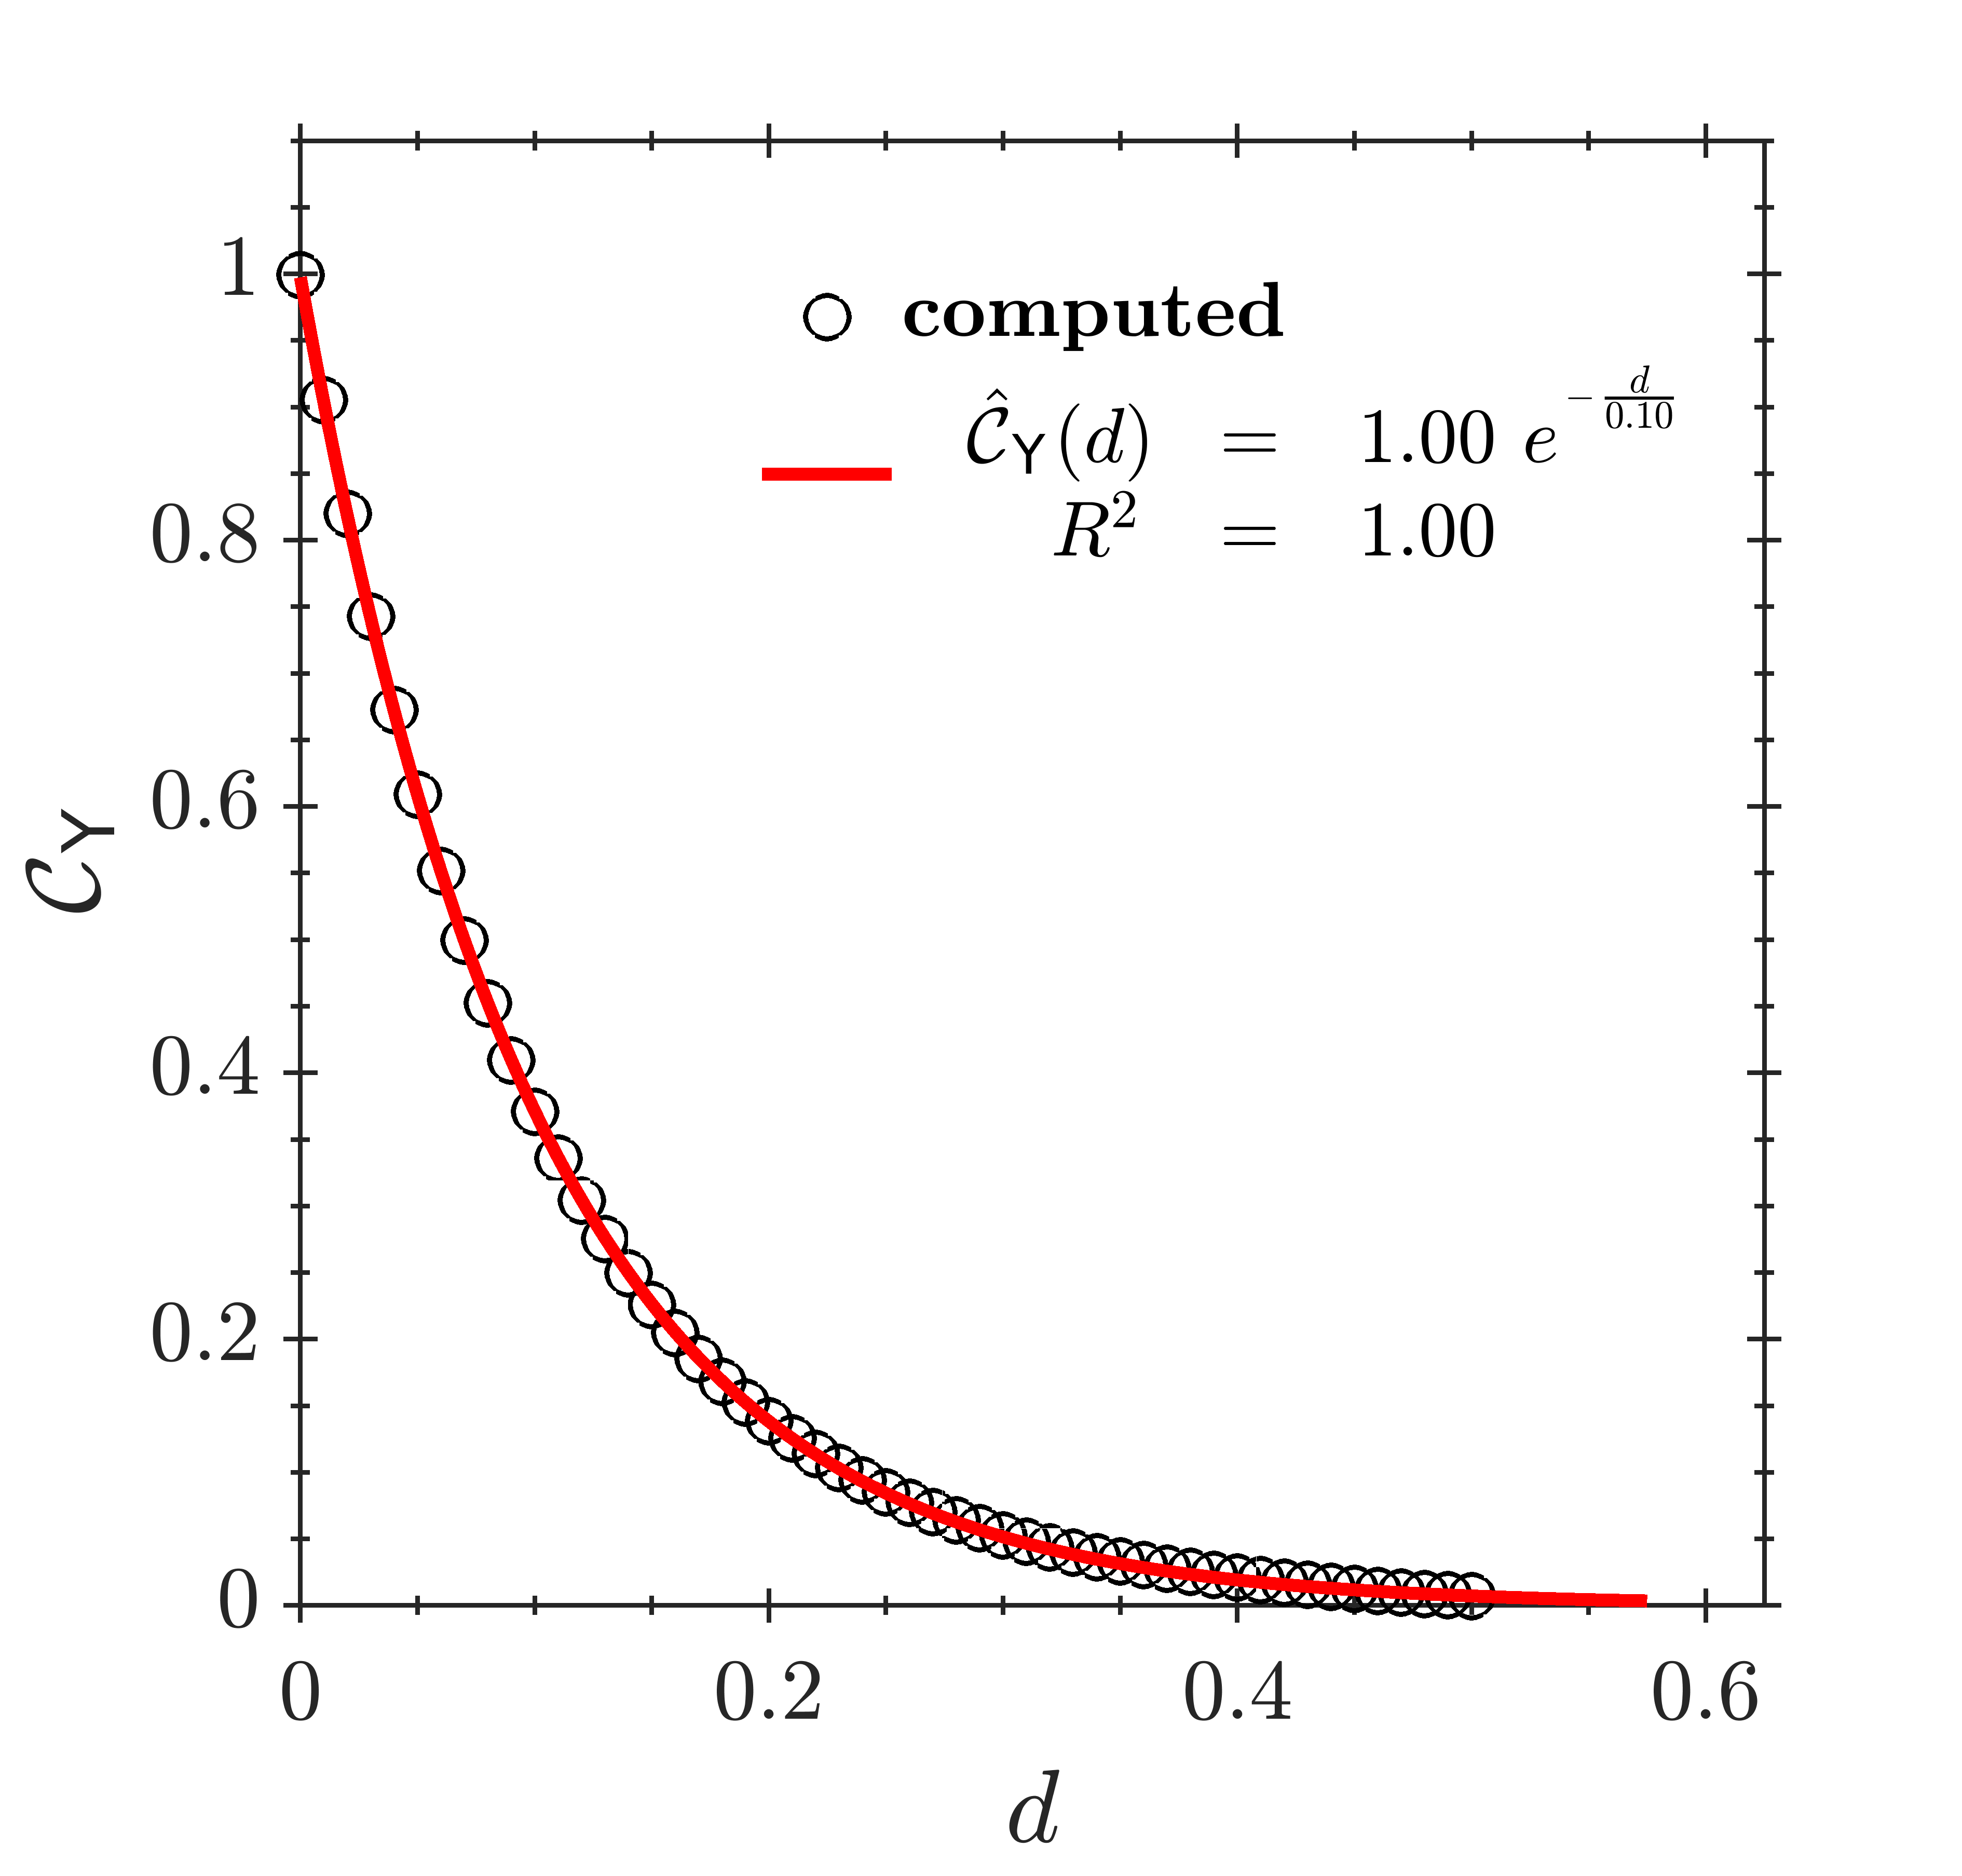
\includegraphics[scale=0.45]{./figuras/e_gsexp_1x1_100x100_0-1x0-1_5000_Yx.png}}
 \subfigure[$y$ direction]{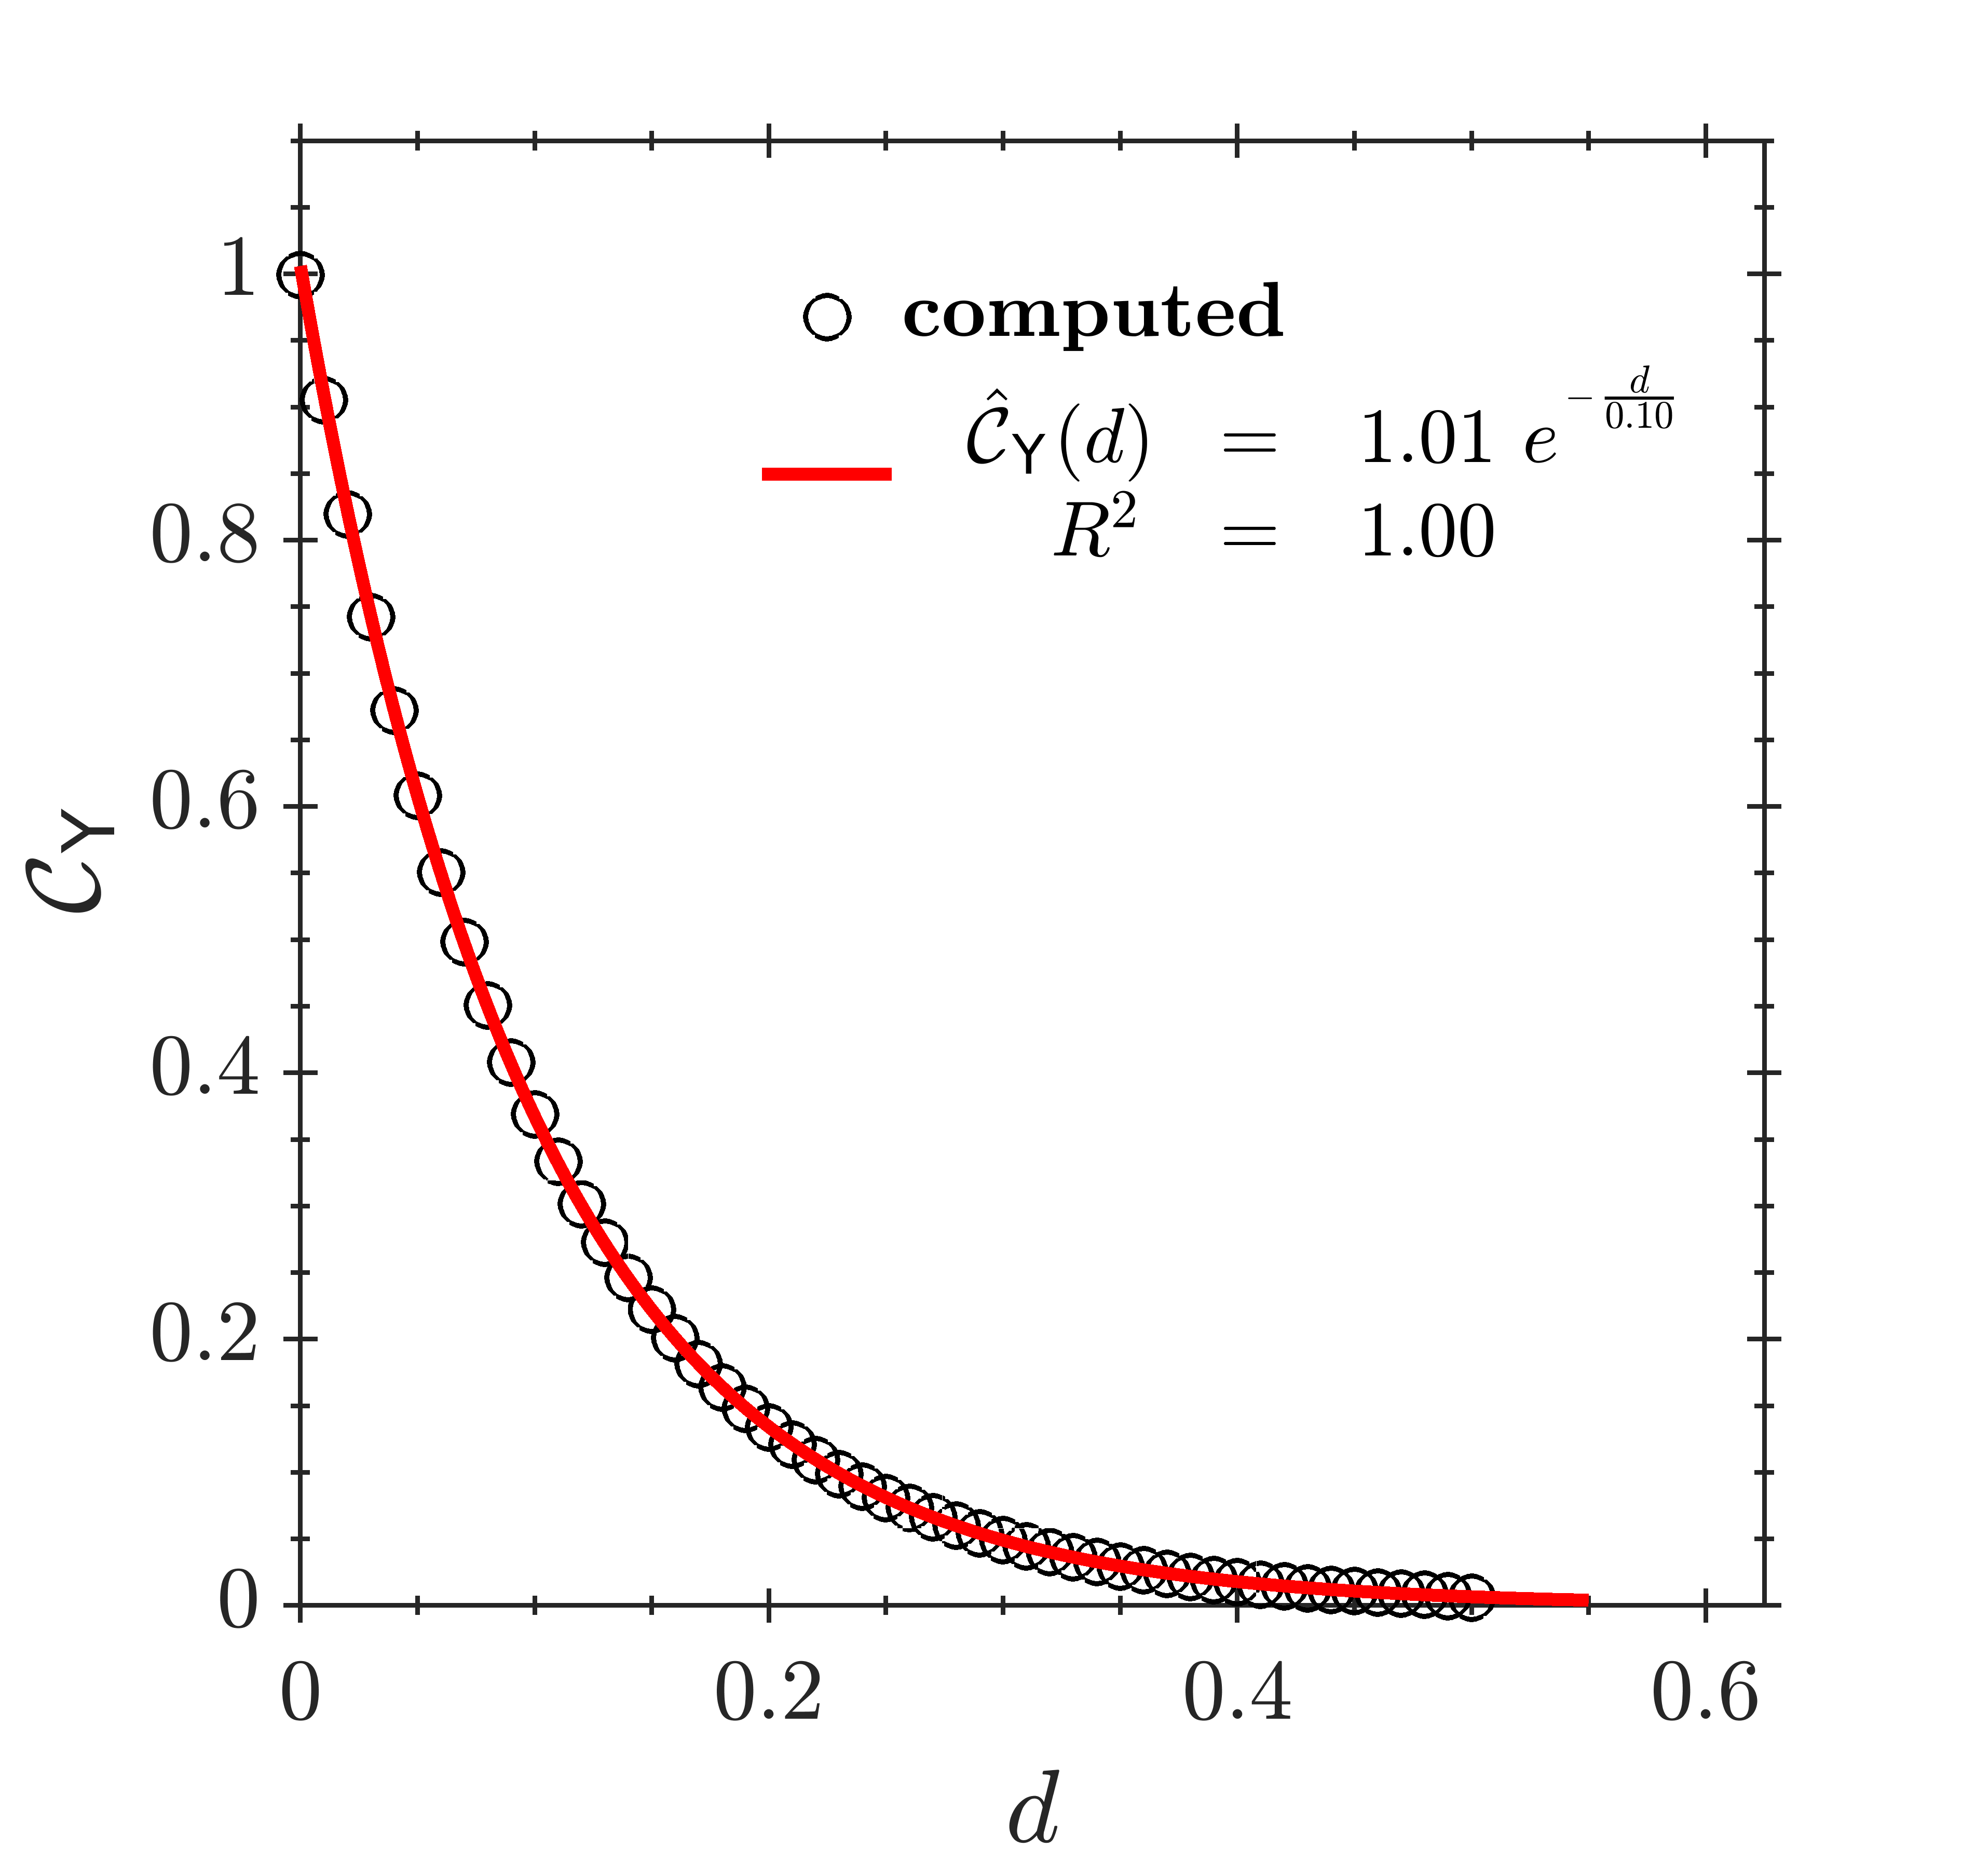
\includegraphics[scale=0.45]{./figuras/e_gsexp_1x1_100x100_0-1x0-1_5000_Yy.png}}
 \caption{Estimated covariance in a sample of $5,000$ fields generate by \kle\ with $30,000$ terms. Exponential case with $\clen = 0.1$.}
 \label{covar_expKL1}
\end{figure}

%%%%%%%%%%%%%%%%%%%%%%%%%%%%%%%%%%%%%%%%%%%%%%%%%%%%%%%%%%%%%%%%%%%%%%%%%%%%%%%%%%%%%%
\begin{figure}[H]
 \centering
 \subfigure[$x$ direction]{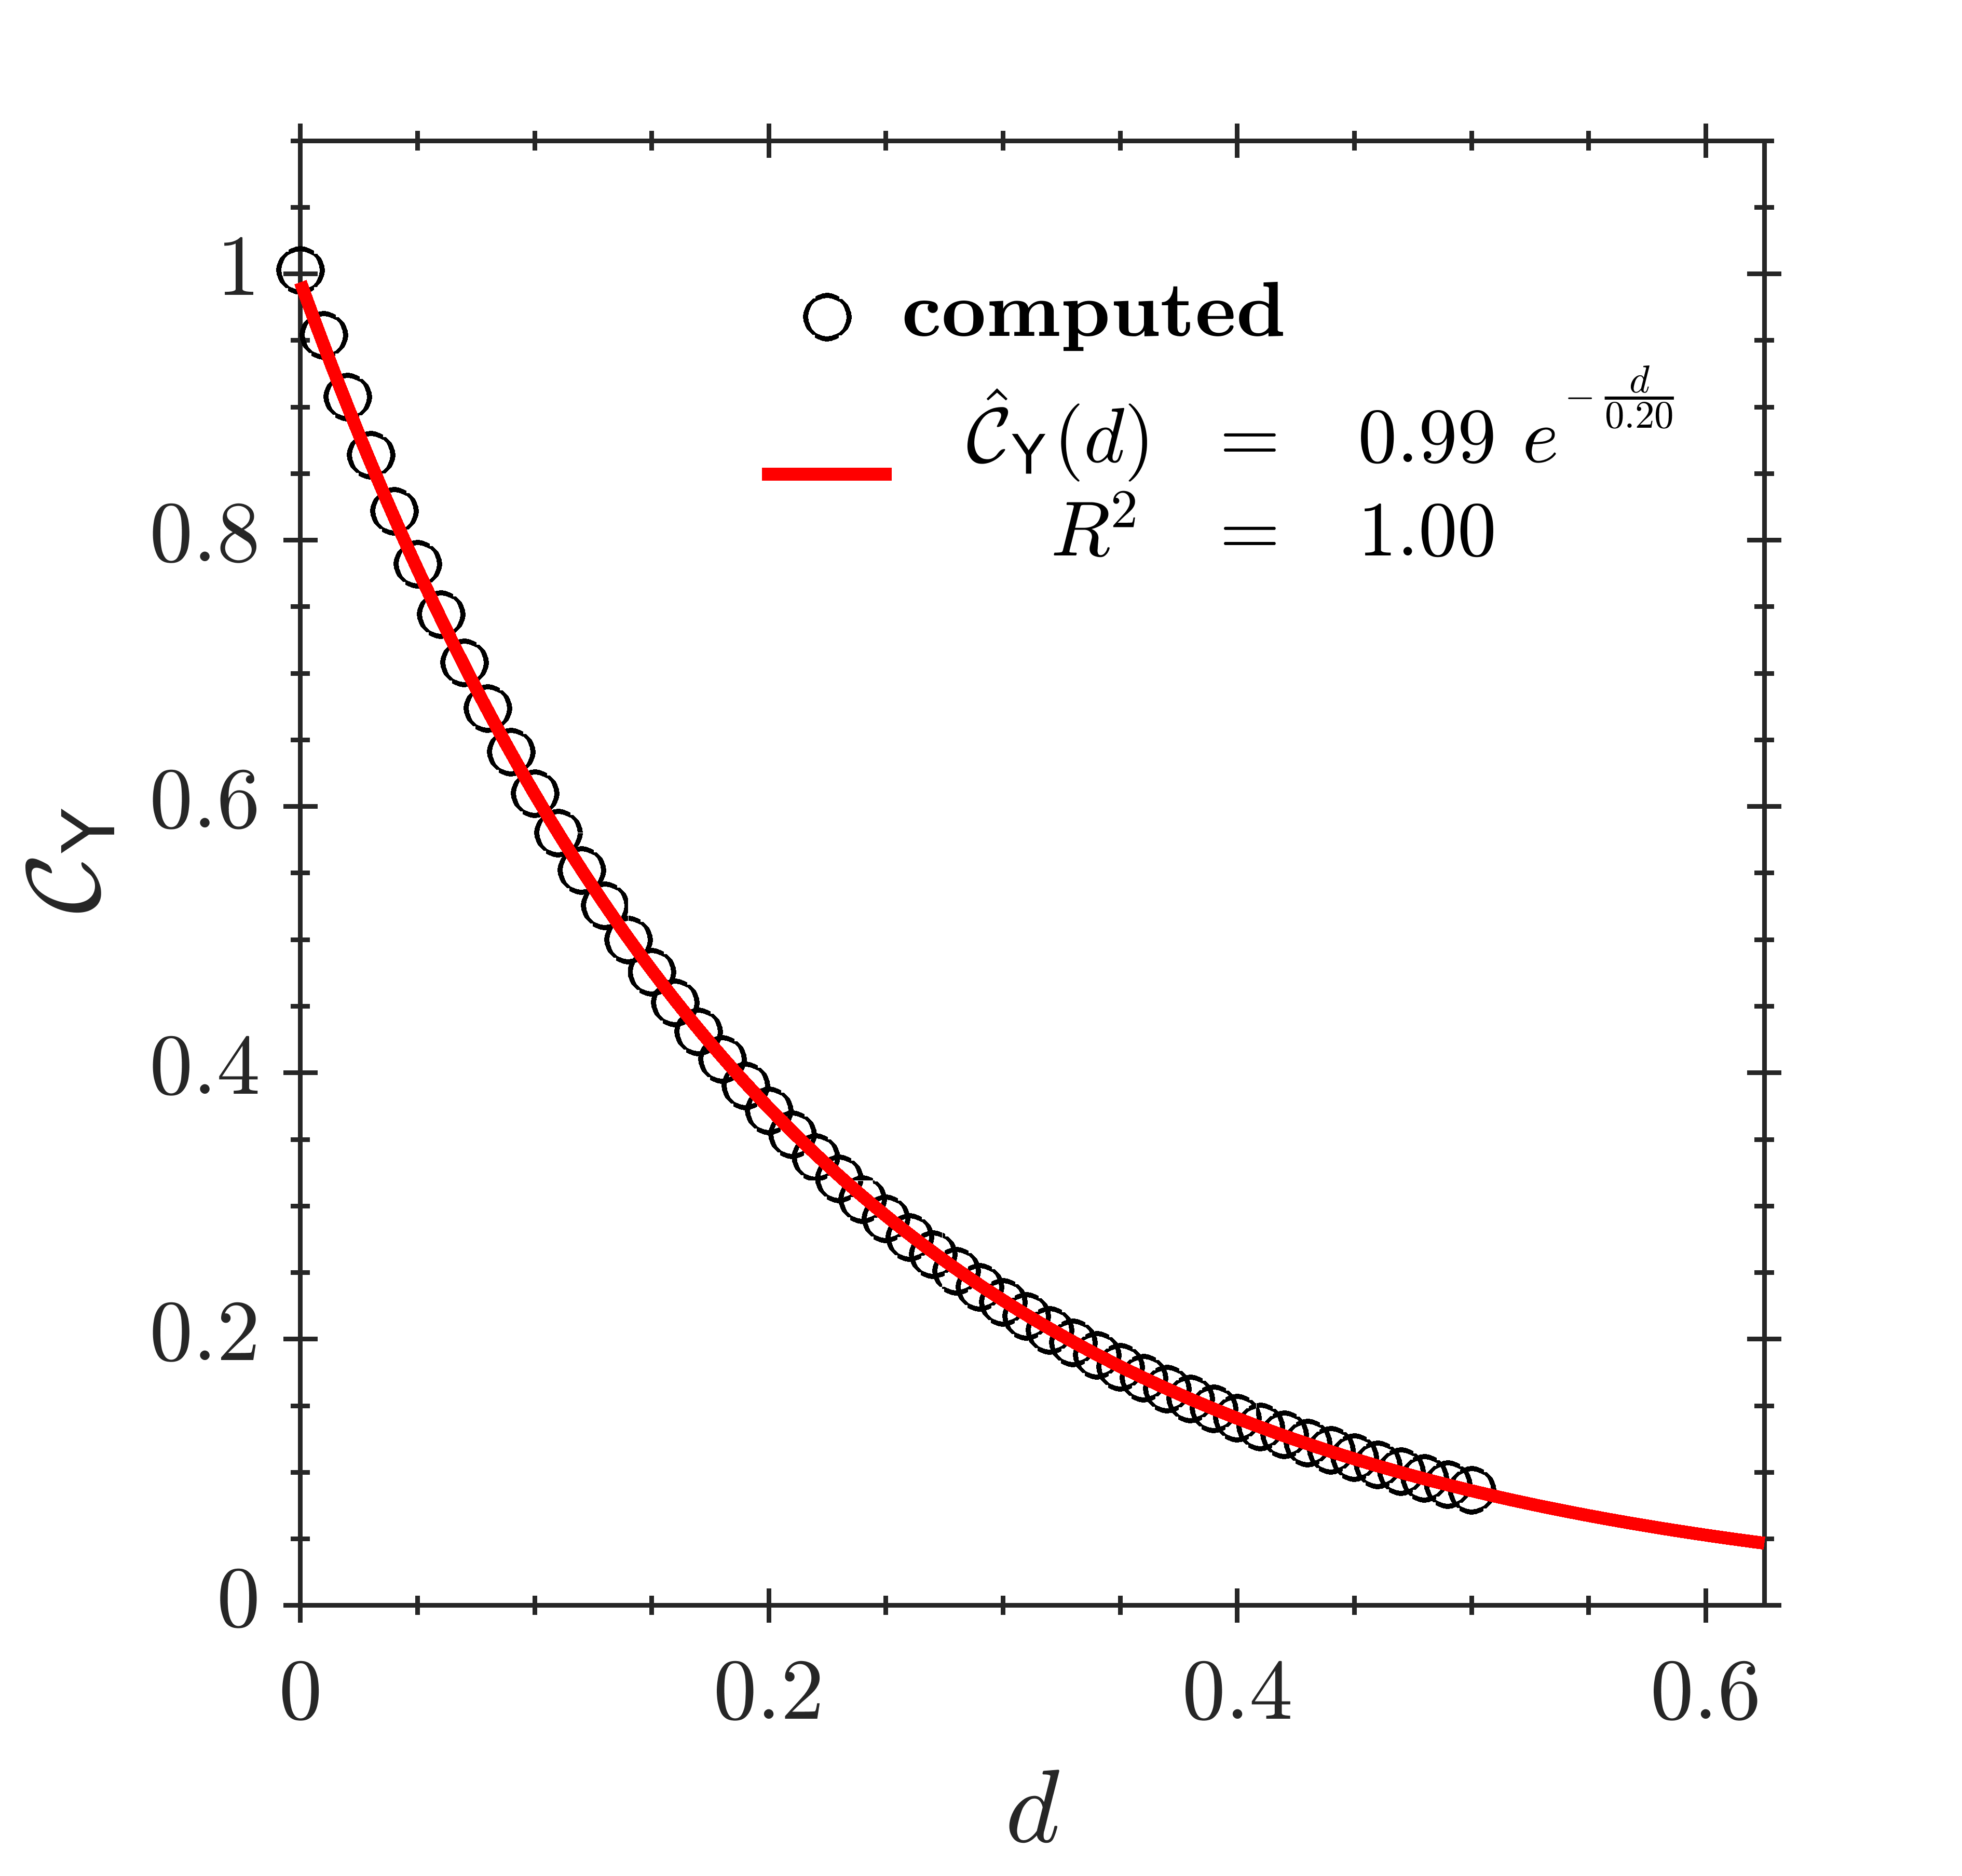
\includegraphics[scale=0.45]{./figuras/e_gsexp_1x1_100x100_0-2x0-2_5000_Yx.png}}
 \subfigure[$y$ direction]{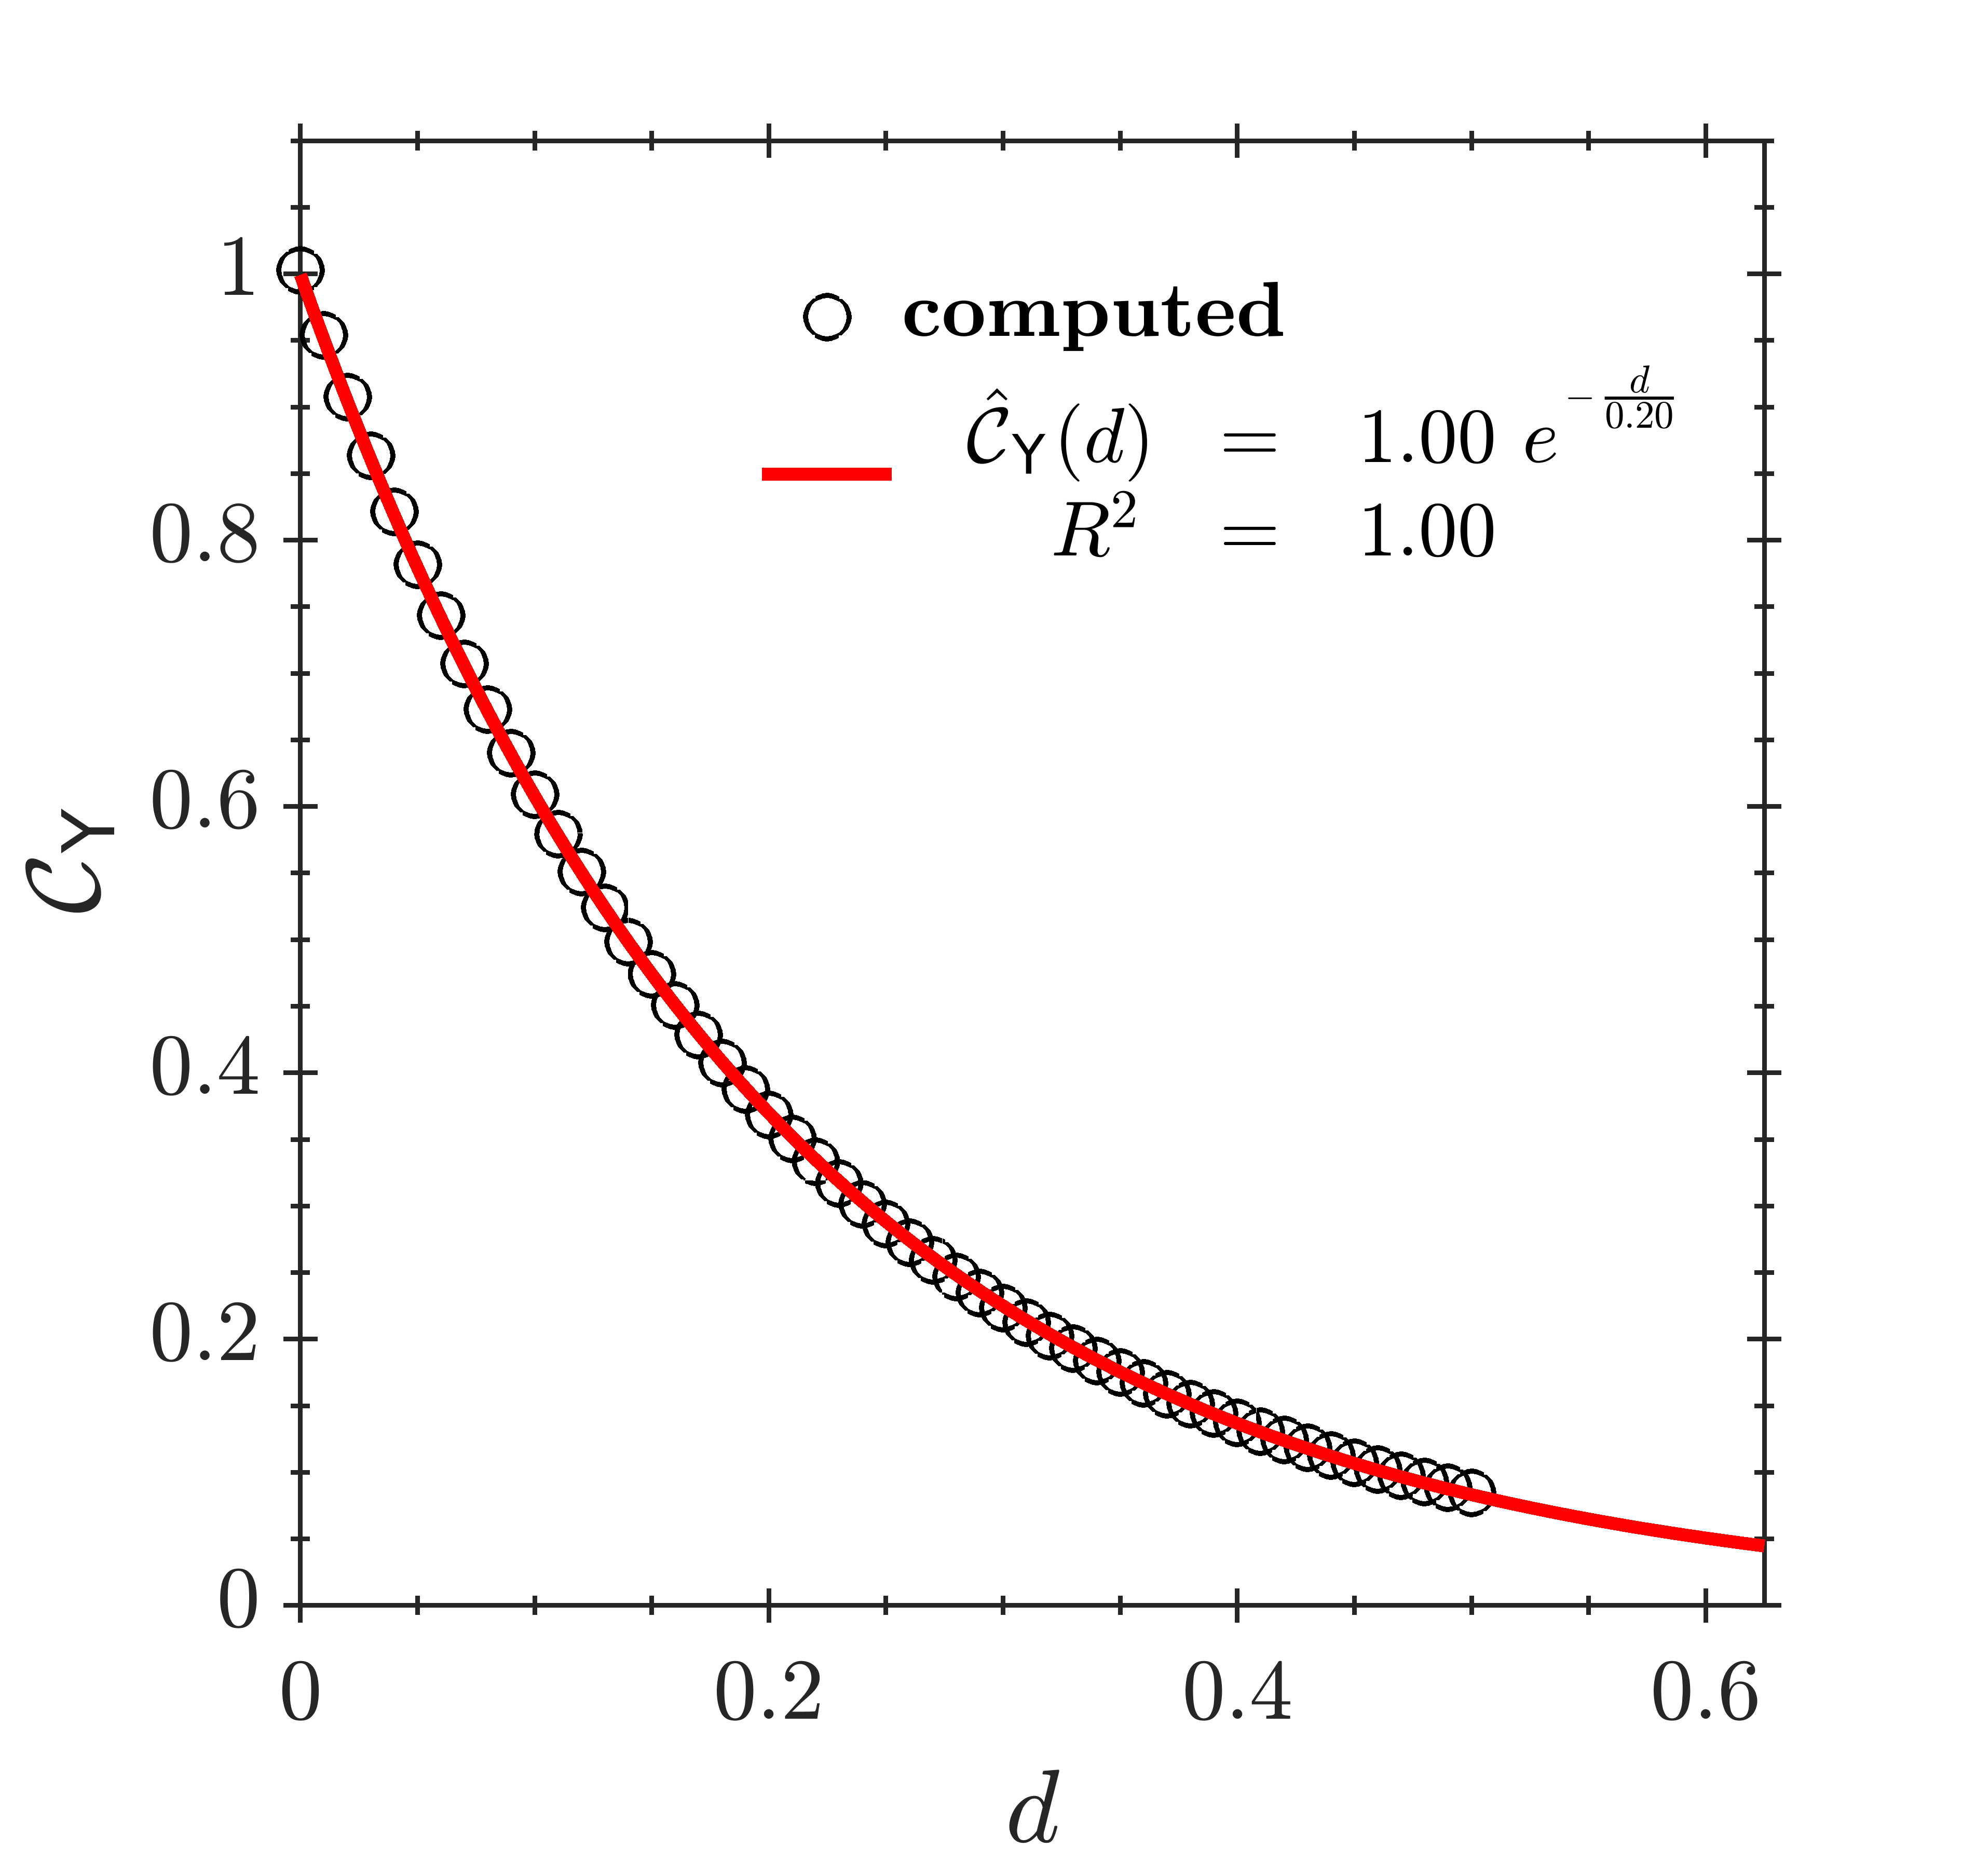
\includegraphics[scale=0.45]{./figuras/e_gsexp_1x1_100x100_0-2x0-2_5000_Yy.png}}
 \caption{Estimated covariance in a sample of $5,000$ fields generate by \kle\ with $30,000$ terms. Exponential case with $\clen = 0.2$.}
 \label{covar_expKL2}
\end{figure}

%%%%%%%%%%%%%%%%%%%%%%%%%%%%%%%%%%%%%%%%%%%%%%%%%%%%%%%%%%%%%%%%%%%%%%%%%%%%%%%%%%%%%%
%%%%%%%%%%%%%%%%%%%%%%%%%%%%%%%%%%%%%%%%%%%%%%%%%%%%%%%%%%%%%%%%%%%%%%%%%%%%%%%%%%%%%%
%%%%%%%%%%%%%%%%%%%%%%%%%%%%%%%%%%%%%%%%%%%%%%%%%%%%%%%%%%%%%%%%%%%%%%%%%%%%%%%%%%%%%%
%%%%%%%%%%%%%%%%%%%%%%%%%%%%%%%%%%%%%%%%%%%%%%%%%%%%%%%%%%%%%%%%%%%%%%%%%%%%%%%%%%%%%%
%%%%%%%%%%%%%%%%%%%%%%%%%%%%%%%%%%%%%%%%%%%%%%%%%%%%%%%%%%%%%%%%%%%%%%%%%%%%%%%%%%%%%%
%%%%%%%%%%%%%%%%%%%%%%%%%%%%%%%%%%%%%%%%%%%%%%%%%%%%%%%%%%%%%%%%%%%%%%%%%%%%%%%%%%%%%%
%%%%%%%%%%%%%%%%%%%%%%%%%%%%%%%%%%%%%%%%%%%%%%%%%%%%%%%%%%%%%%%%%%%%%%%%%%%%%%%%%%%%%%
%%%%%%%%%%%%%%%%%%%%%%%%%%%%%%%%%%%%%%%%%%%%%%%%%%%%%%%%%%%%%%%%%%%%%%%%%%%%%%%%%%%%%%
